\chapter{Forecasting the daily electricity consumption}
\label{cha:Forecasting the daily electricity consumption}
In this chapter different forecasting techniques to perform 24 hours ahead predictions for individual household electrical consumption are discussed. The time series have a half hourly frequency, which means that $ 48 $ data points have to be estimated during each prediction of a day. The day we want to forecast is further indicated as the ``desired day''. First the raw data is introduced and preprocessing steps done are explained in Section \ref{s:Preprocessing}. Section \ref{s:Baseline models} presents the baseline models. These models are implemented using a straightforward approach. They serve as a benchmark for more complex models in Section \ref{s:Neural network models}. ``Long Short-Term Memory'' neural networks are most suitable to process time series and have therefore been chosen as the core model which is analysed with different design choices. Finally, a parameter search is conducted which consists of analysing the best parameters for optimal results.
 
\section{Preprocessing}\label{s:Preprocessing}
The available raw data is summarized by Table \ref{tab:available_data}. 
Three series are selected from the \textit{consumption.csv} for which the important characteristics are summarized by Table \ref{tab:summ_data}. The chosen time series have the least amount of missing data and don't contain large shifts of the mean consumption during the year. Figure \ref{fig:three_series} shows the electrical consumption of the three selected series. The validation set used during the parameter search consists out of the $ 10 $ last days in November. Only $ 10 $ days are selected to reduce the amount of predictions the models have to calculate. Also, these days don't contain any missing values for the three series. The months January till  November compose the training set and December is taken as test set.\\ 
The corresponding average temperature series are also used. They don't contain any missing values.

\begin{figure}[ht]
	\begin{subfigure}{0.32\textwidth}
		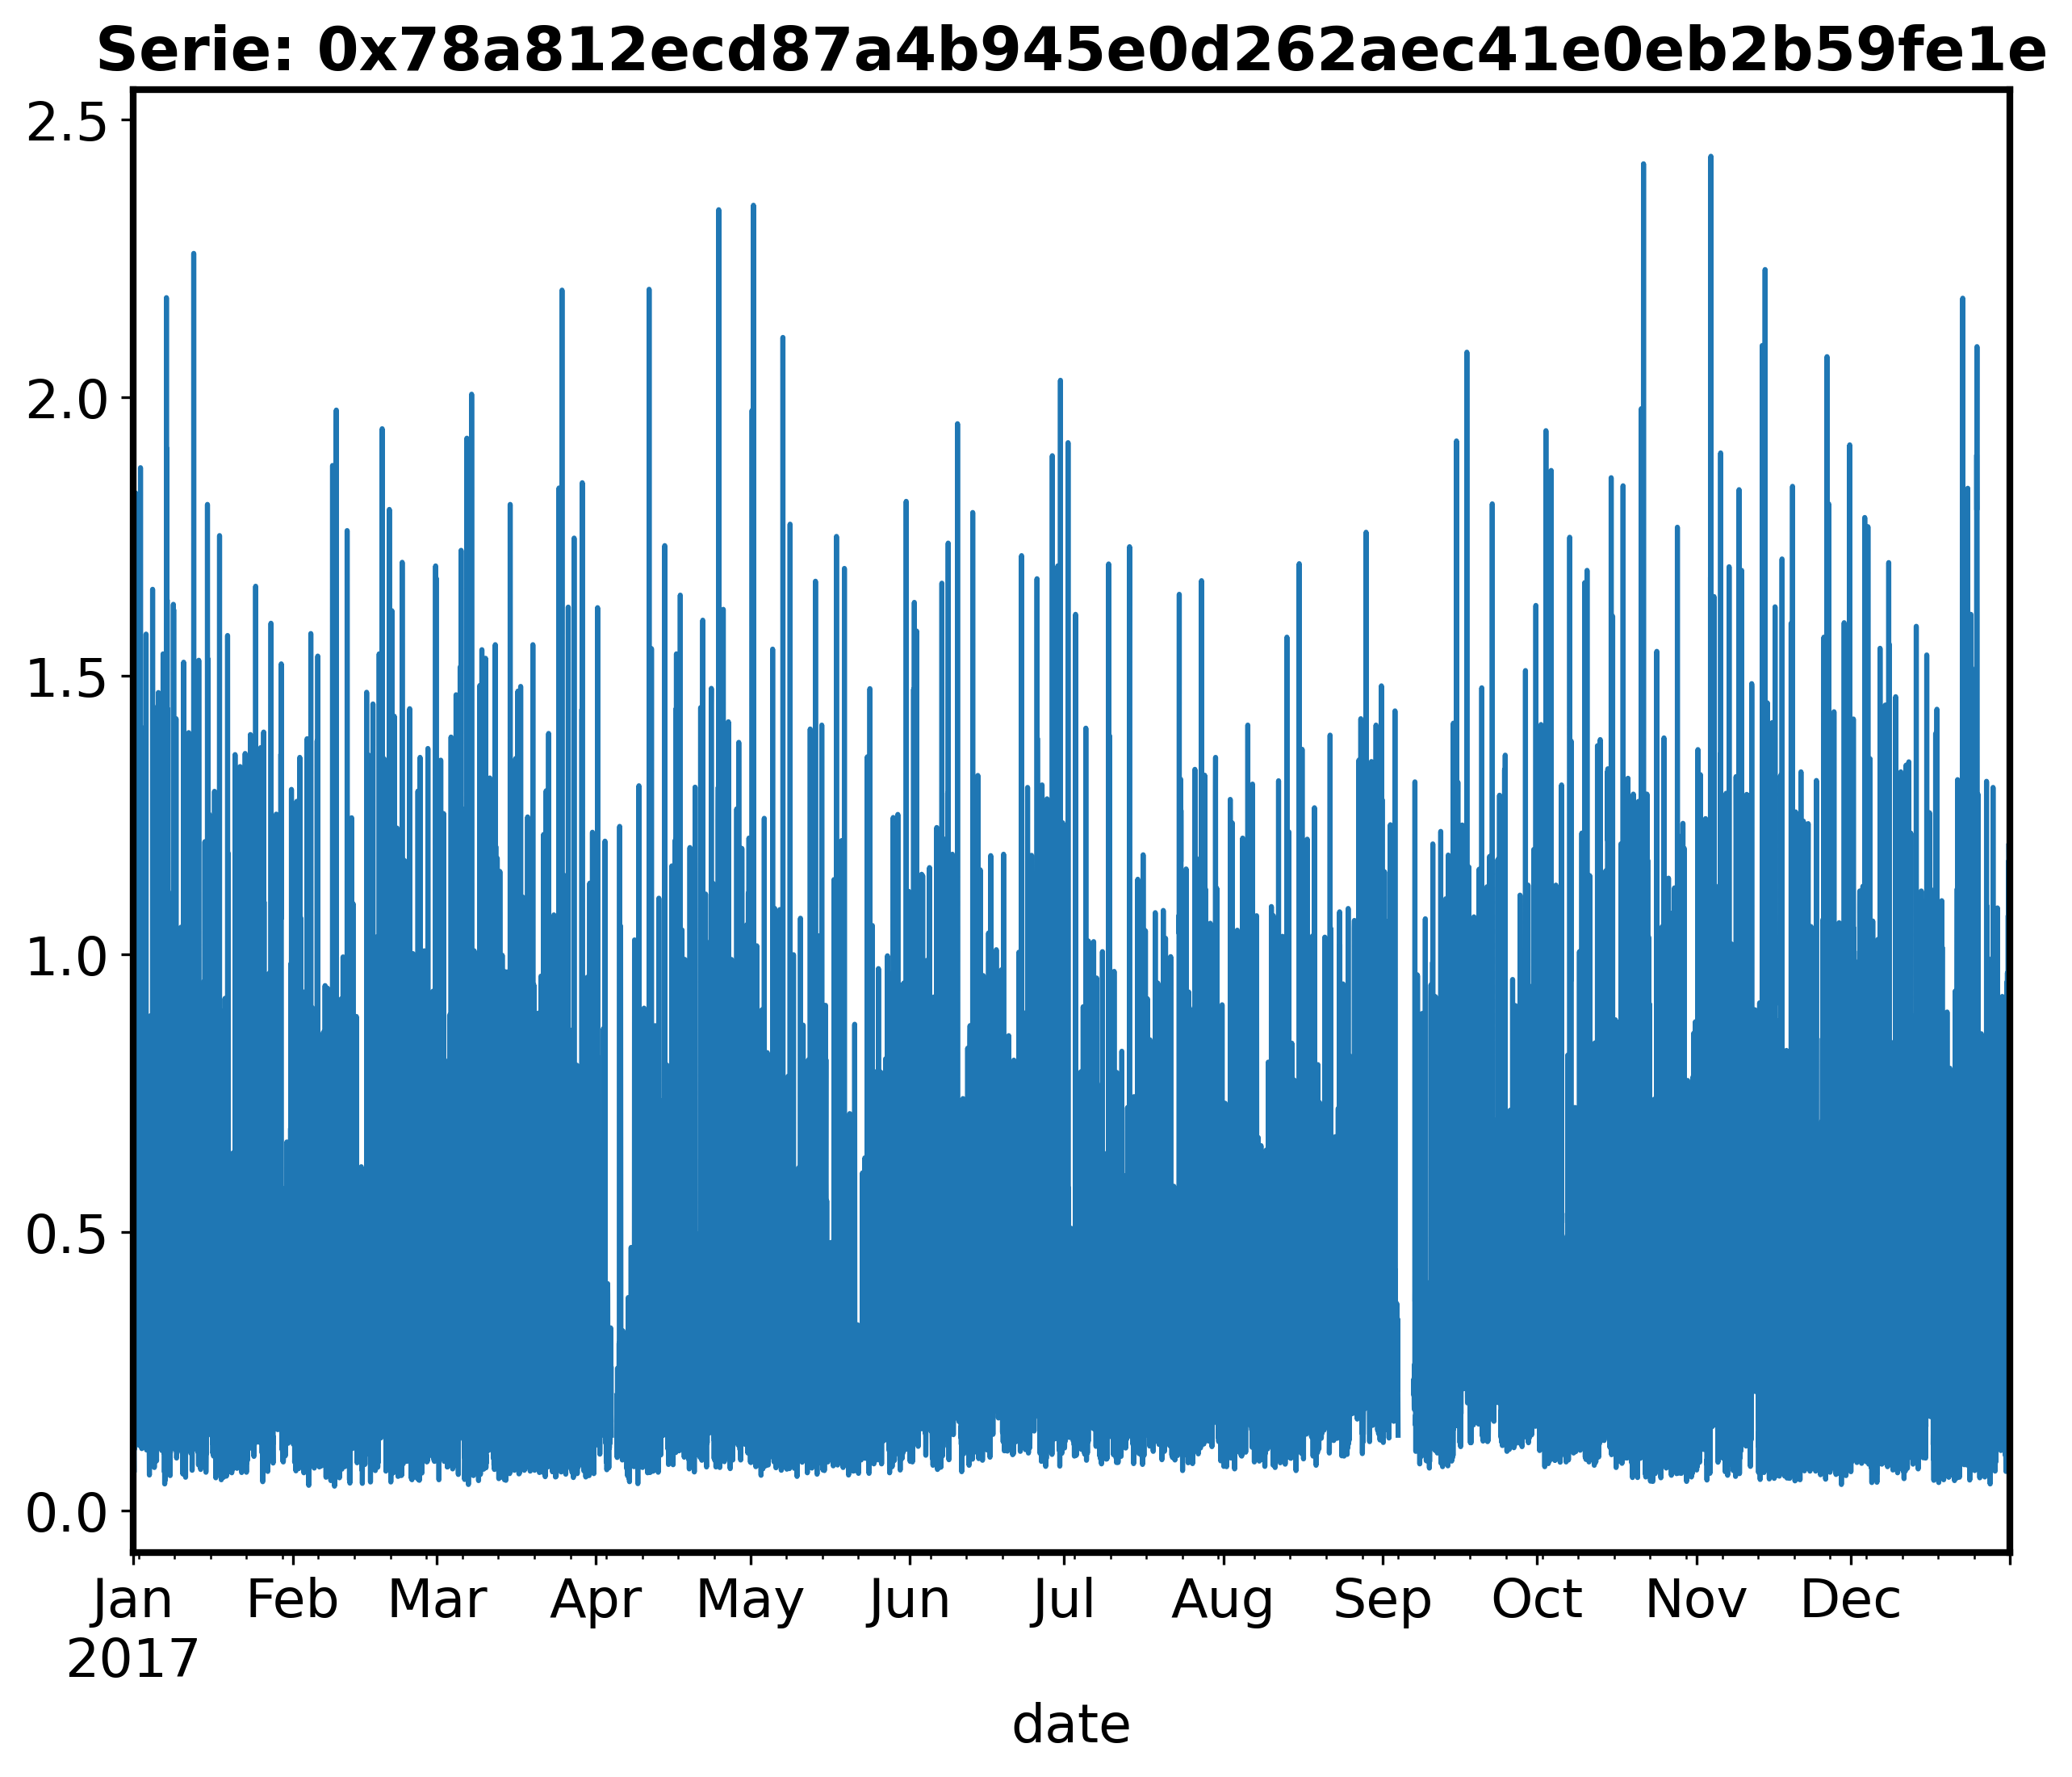
\includegraphics[width=1\linewidth]{Serie0x78a812ecd87a4b945e0d262aec41e0eb2b59fe1e.png}
		\caption{Serie $ 1 $}
	\end{subfigure}	 	
	\begin{subfigure}{0.32\textwidth}
		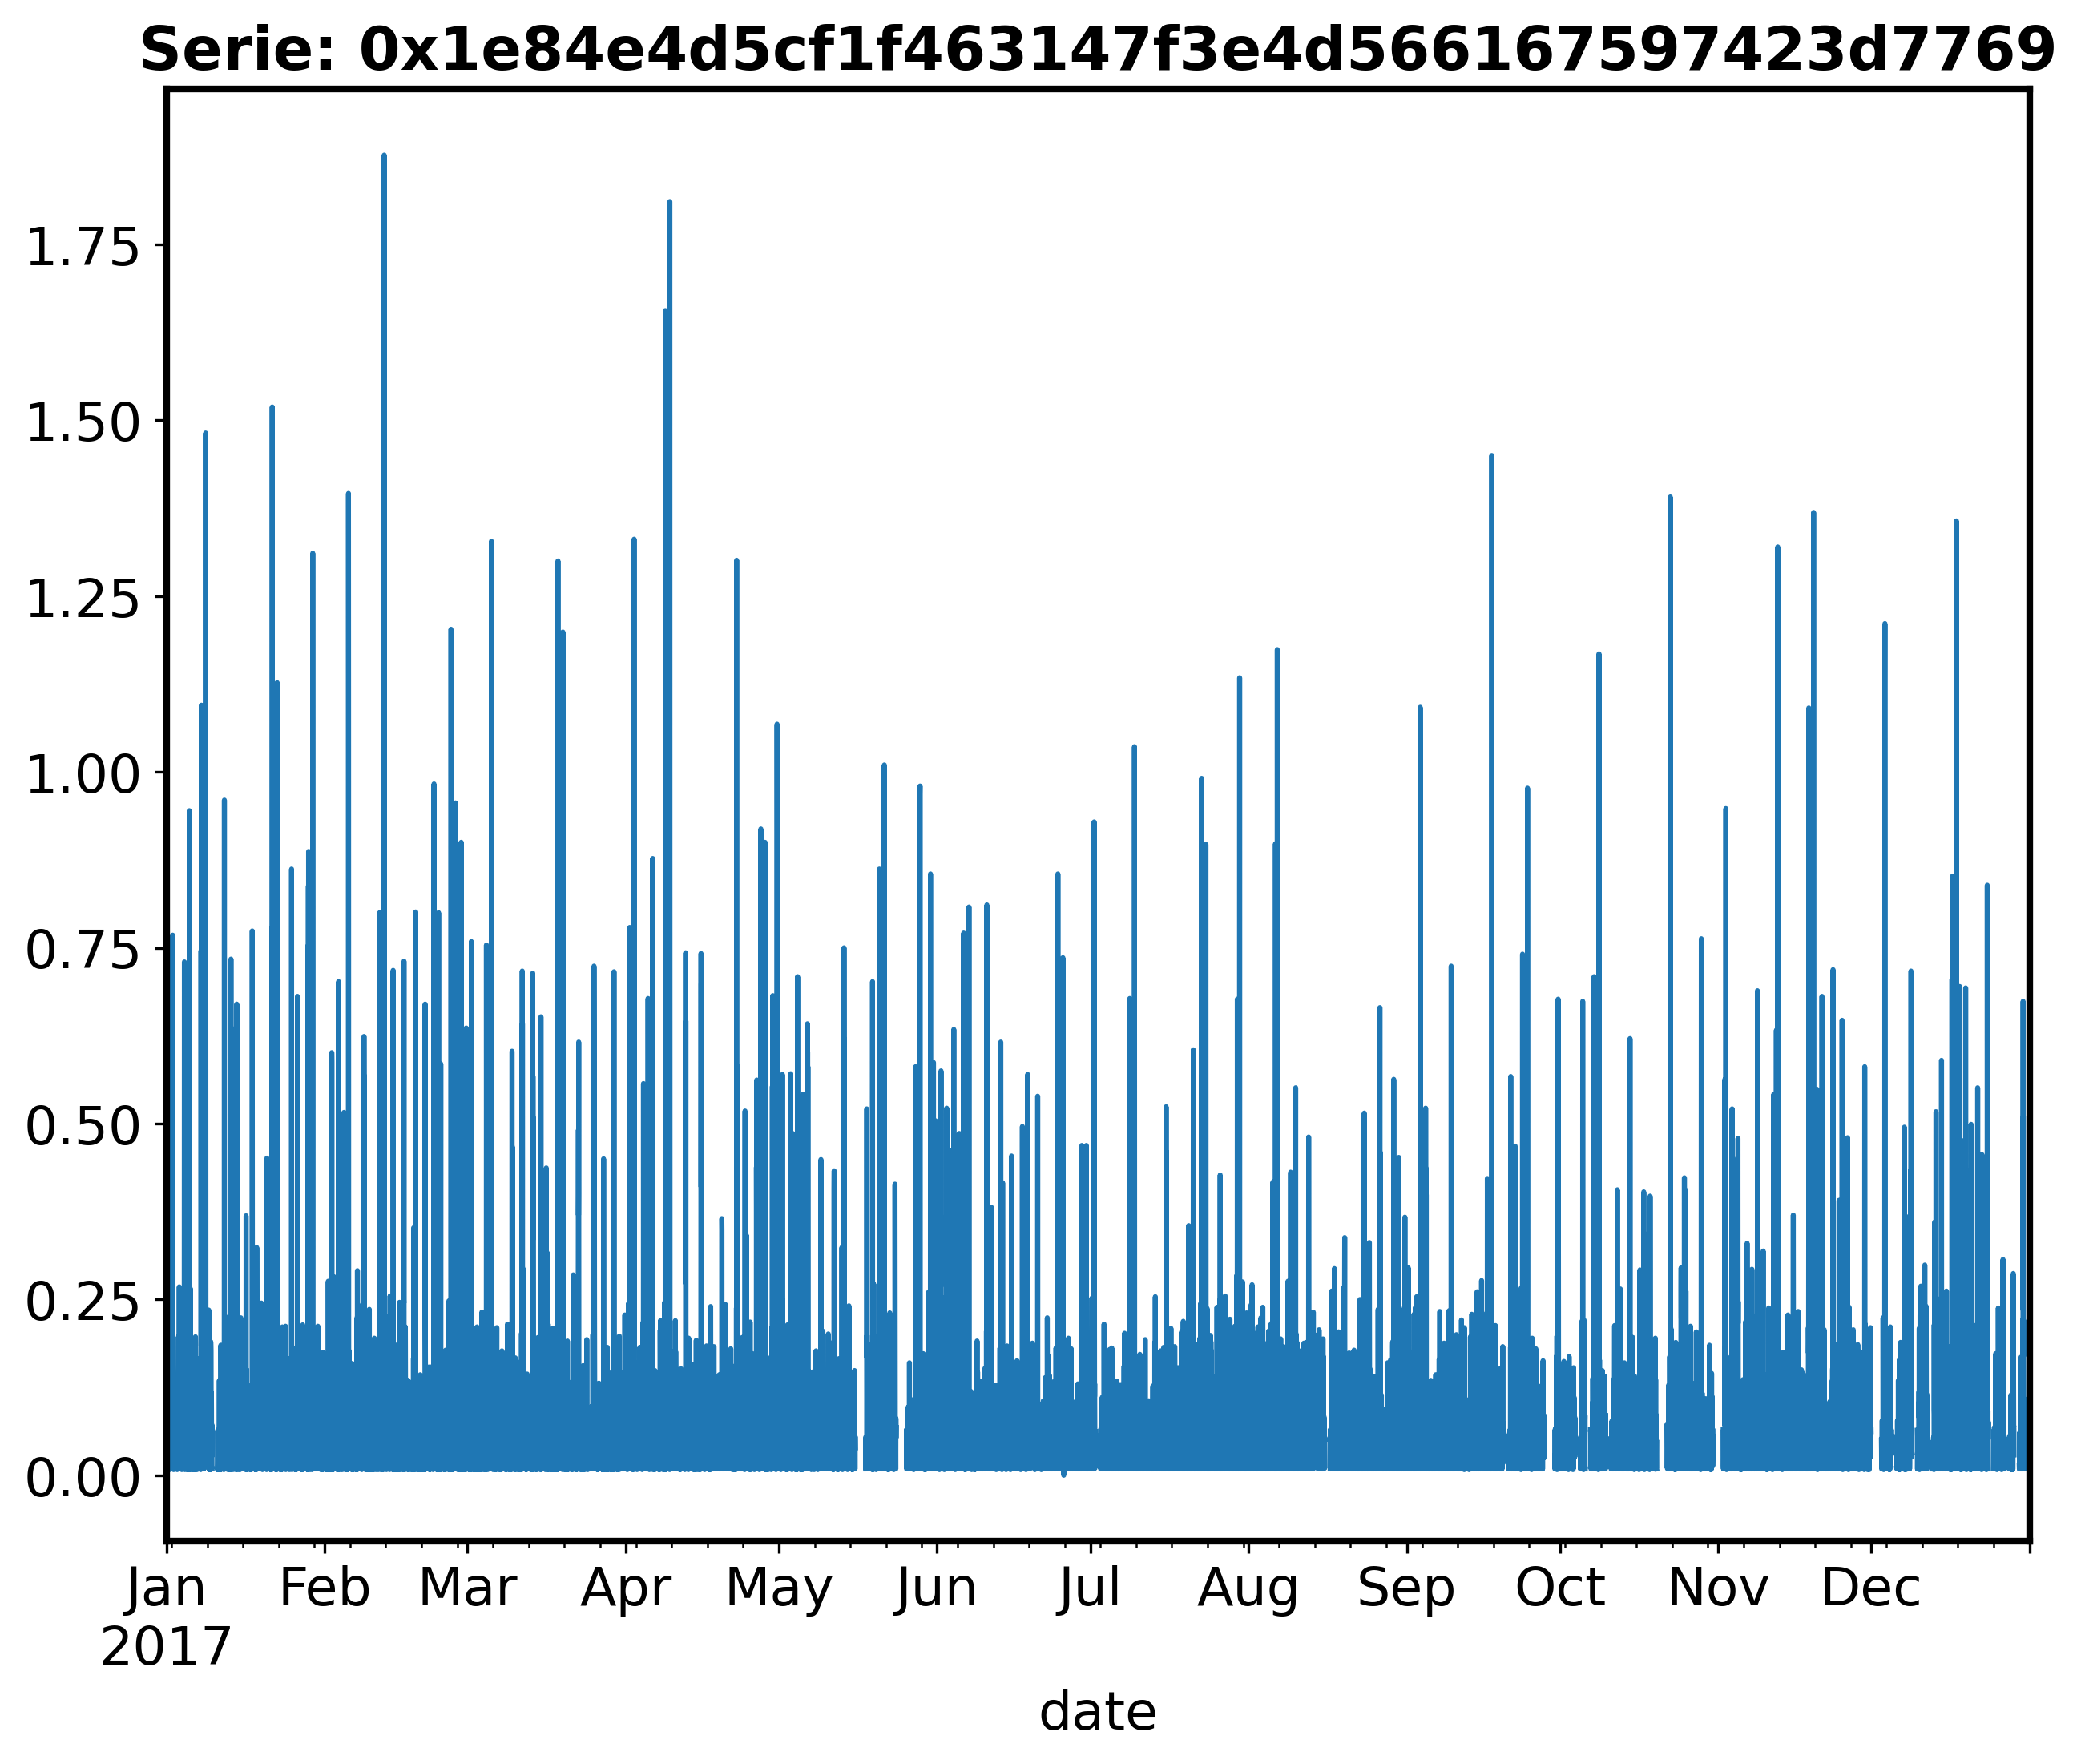
\includegraphics[width=1\linewidth]{Serie0x1e84e4d5cf1f463147f3e4d566167597423d7769.png}
		\caption{Serie $ 2 $}
	\end{subfigure}	
	\begin{subfigure}{0.32\textwidth}
		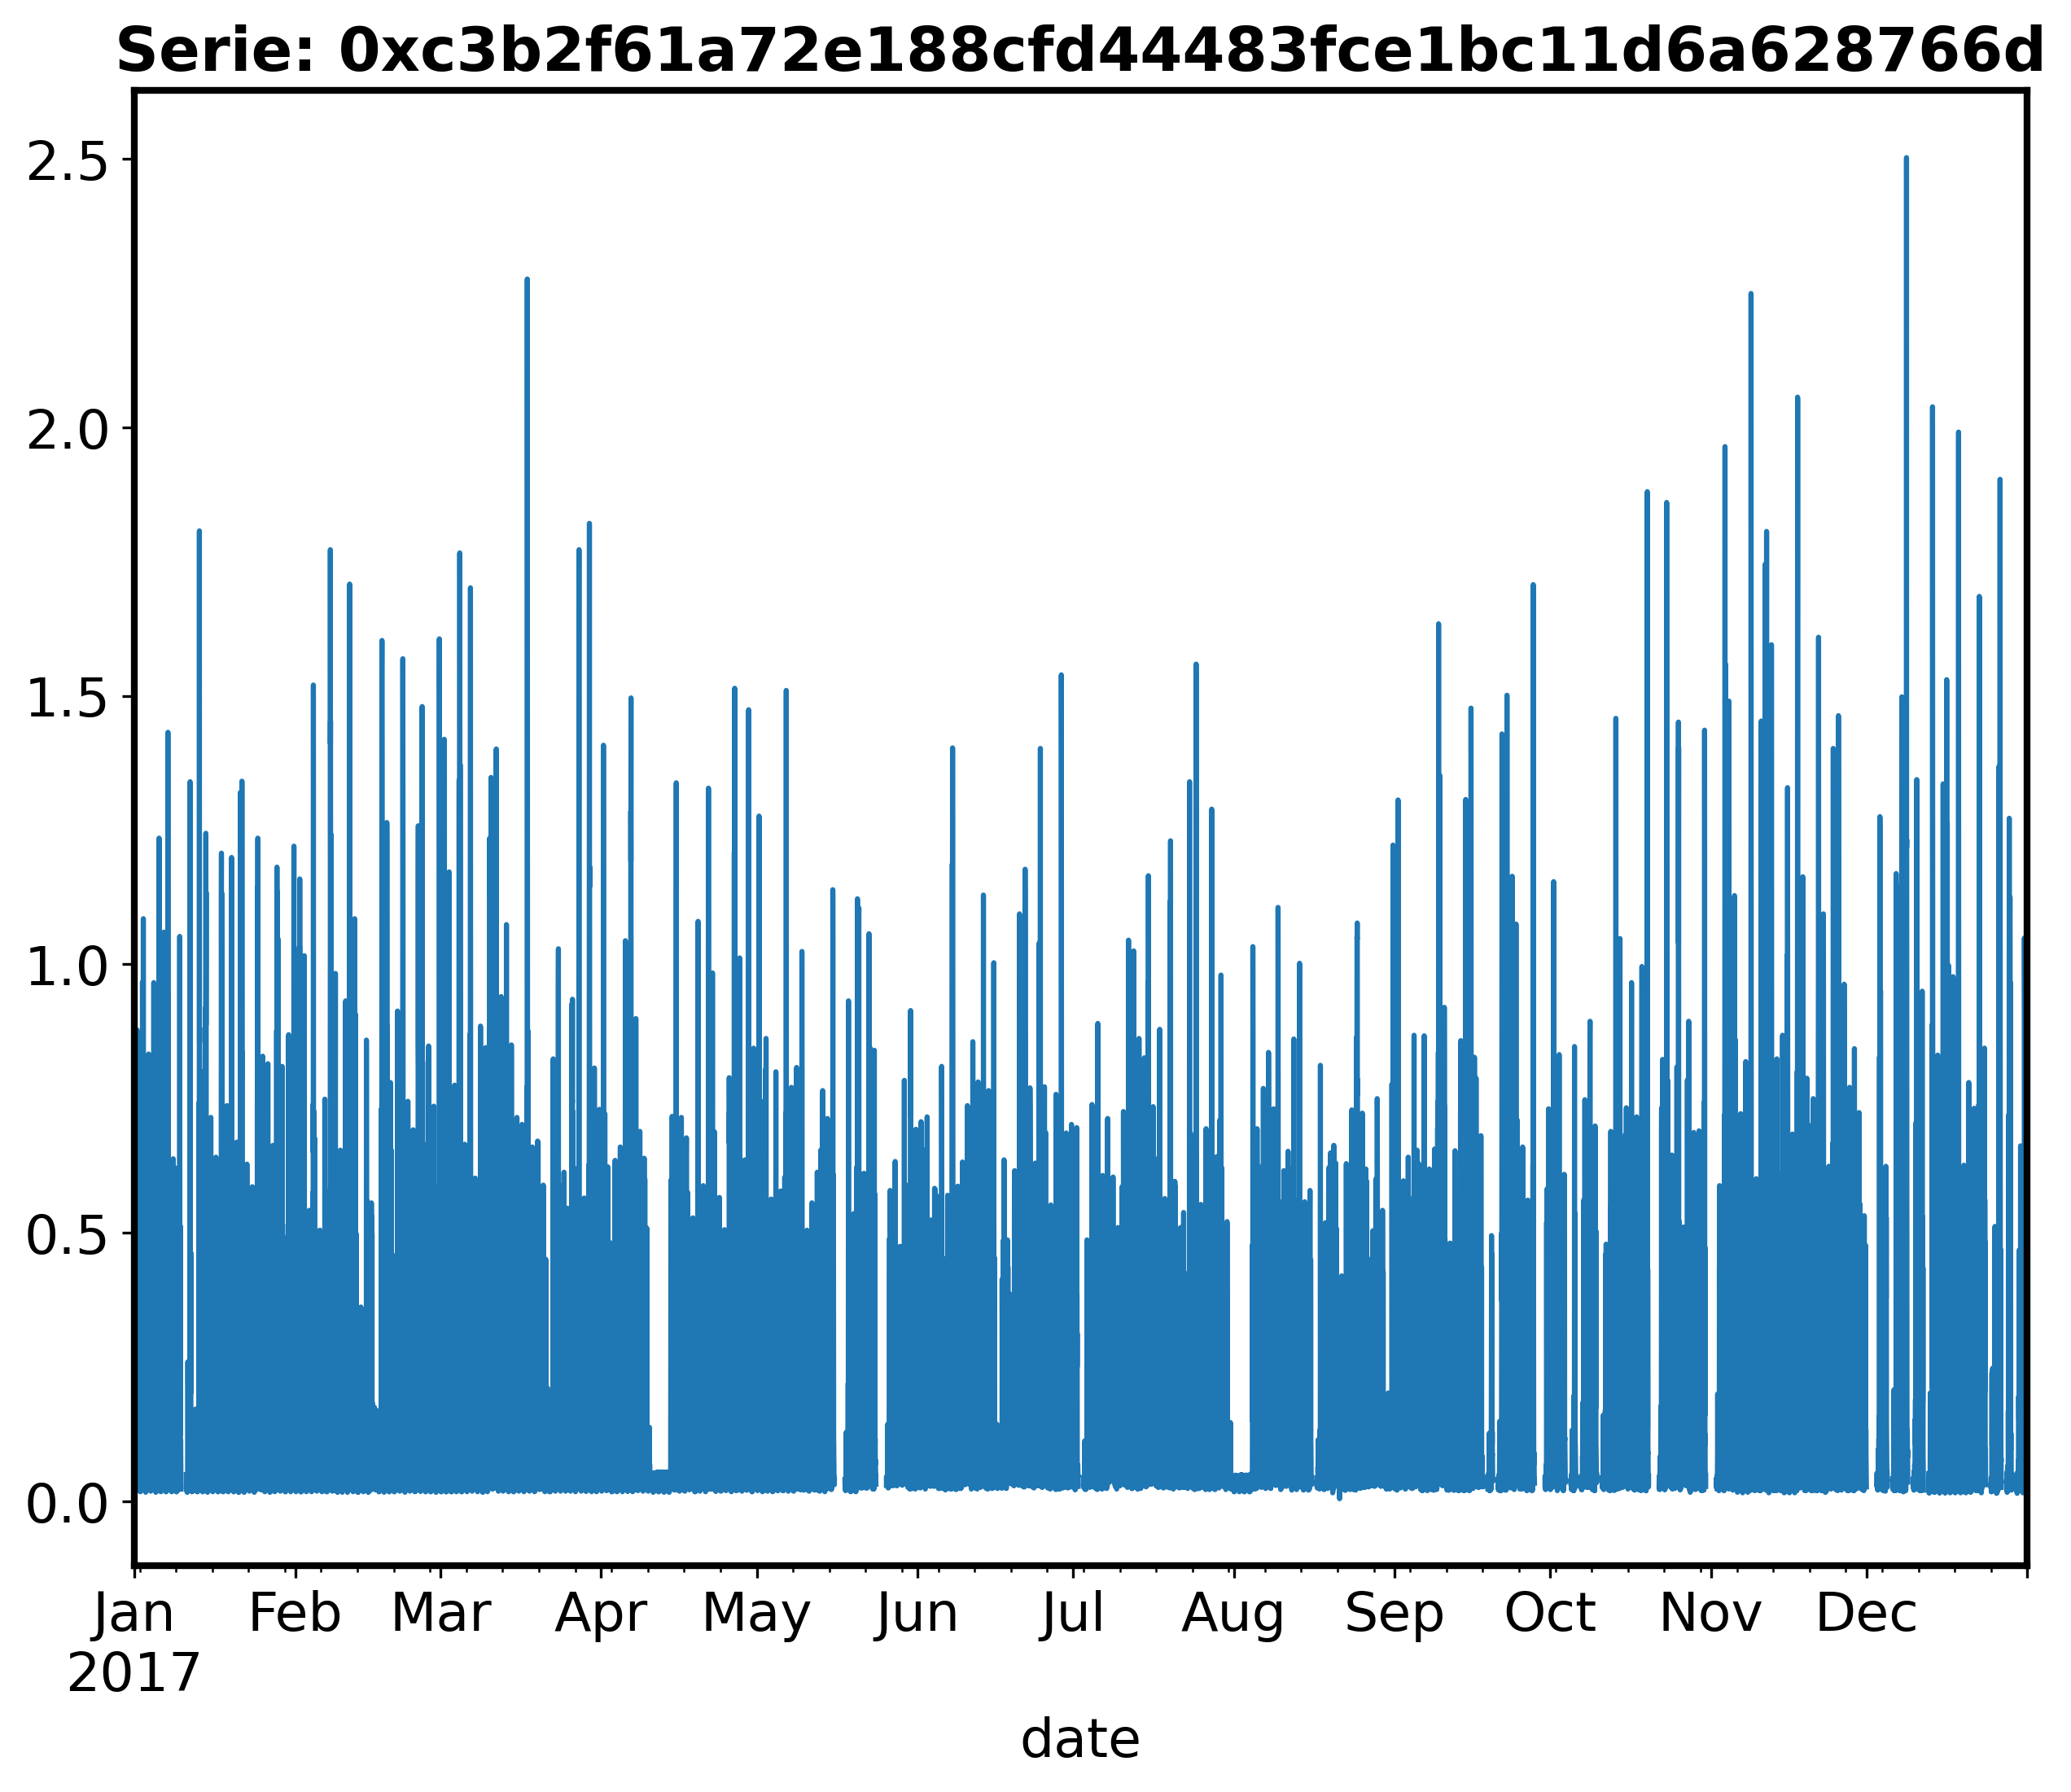
\includegraphics[width=1\linewidth]{Serie0xc3b2f61a72e188cfd44483fce1bc11d6a628766d.png}
		\caption{Serie $ 3 $}
	\end{subfigure}
	\caption{The electrical consumption in $ 2017 $ for the three selected series. }
	\label{fig:three_series}
\end{figure}

\begin{table}
  \centering
  \begin{tabular}{@{}l|llr@{}} \toprule
  	\textbf{Characteristic}	& \textbf{Serie $ 1 $} & \textbf{Serie $ 2 $} & \textbf{Serie $ 3 $}\\\midrule
    Mean daily consumption [kWh]& $ 14.55 $&$ 3.17 $  & $ 6.58 $ \\
    Standard deviation daily consumption [kWh] &$ 3.21 $ & $ 0.99 $& $ 2.57 $ \\
    Median daily consumption [kWh] & $ 14.09 $ & $ 2.96 $& $ 5.88 $ \\
    Maximum daily consumption [kWh] & $ 30.08 $ & $ 6.60 $ &  $ 17.15 $   \\
    Minimum daily consumption [kWh]& $ 7.51 $ & $ 1.83 $ &  $ 1.50 $   \\
    Total missing days (consumption) & $ 4 $ &$ 25 $ & $ 26 $\\
    Days in validation set (21-30 November)&  $ 10 $ & $ 10 $  & $ 10 $ \\
    Days in Test set (December) & $ 31 $    &    $ 23 $  & $ 23 $ \\
    Days in training set (Rest)&   $ 320 $  &  $ 307 $   &  $ 306 $\\
    Mean average temperature [$\degree C$]& $ 10.37 $  &  $ 10.61 $  & $ 10.22 $ \\
    Standard deviation average temperature [$\degree C$]& $ 5.09 $  & $ 5.20 $   & $ 5.01 $ \\
    Median average temperature [$\degree C$] &  $ 10.46 $ &  $ 10.61 $  & $ 10.35 $ \\
    Maximum average temperature [$\degree C$] & $ 23.99 $  & $ 24.51 $   & $ 22.95 $ \\ 
    Minimum average temperature [$\degree C$] & $ -1.07 $  &  $ -1.28 $  & $ -1.42 $ \\
    Missing average temperature days &  $ 0 $ & $ 0 $  & $ 0 $  \\ 
    Amount of holidays in $ 2017 $ & $ 8 $  &  $ 8 $  & $ 8 $ \\\bottomrule
  \end{tabular}
  \caption{Summarizing characteristics about the selected series.}
  \label{tab:summ_data}
\end{table}

During this chapter the series containing the electrical consumption are not aggregated as was the case in Section \ref{s:Analysis}. Therefore, the min-max normalization is a suitable normalization method for each serie. It is chosen to estimate the missing values in the training set and not leave them out. In other words, a larger trainings set with an additional estimation error is preferred. By imputing the missing values more training data is available but also time jumps are avoided. As discussed earlier, data that is missing are always complete days. These are estimated using baseline models that will be discussed in Section \ref{s:Baseline models} in following order: ``previous week forecast'', ``previous day forecast'' and ``mean forecast''. When the first baseline model can't make a prediction for the missing day i.e. the day during previous week is not available, the next baseline model is used and so on.\\

\section{Error metrics}
The metrics that can be used to evaluate the performance of predictions are  RMSE (Eq. \ref{eq:RMSE}), NRMSE (Eq. \ref{eq:NRMSE}),  MAE  (Eq. \ref{eq:MAE}),  MSE (Eq. \ref{eq:MSE}) and MAPE (Eq. \ref{eq:MAPE}).

\begin{equation}\label{eq:MSE}
	MSE = \frac{\sum_{t=1}^{N}(\hat{y}_t-y_t)^2}{N}
\end{equation}

\begin{equation}\label{eq:MAPE}
	MAPE = \frac{\sum_{t=1}^{N}\abs{\hat{y}_t-y_t}/y_t}{N}
\end{equation}


It is expected that the \textit{MAE} penalizes outliers less severe than \textit{MSE}, which takes the error squared. Therefore, using the \textit{MSE} metric, more emphasize is put on predicting the peaks of the reference signal correctly with respect to \textit{MAE}. The advantage of using  RMSE  and MAE  is that they both have an error in kWh which is intuitive.  NRMSE  and  MAPE  take the reference signal into account. NRMSE  gives a bigger error, when the reference signal has a small difference between the $ y_{max} $ and $ y_{min} $.  MAPE  penalizes a small MAE more severe on a small reference value than on a larger one due to the division by $ y $.


\section{Microsoft Azure cloud}
The calculations executed in this chapter are performed on a virtual machine using the Microsoft Azure services. This was possible because Microsoft provides students with $ \$ 100 $ of free credit. Table \ref{tab:CPU} shows the different features of the CPU/GPU's used during this thesis. 

\begin{table}[hb]
	\centering
	\begin{tabular}{|p{5cm}||p{2cm}|p{2cm}|p{2cm}|p{2cm}|}\hline
		\textbf{Name}	& \textbf{Logical cores} & \textbf{RAM (GB)} & \textbf{Storage (GB)} & \textbf{Cost}\\\hline
		F4s v2 (CPU - Azure)& $ 4 $&$ 8 $  & $ 32 $ & $ \$ 0.194/hour $\\\hline
		NVIDIA Tesla K80 (GPU - Azure)& $ 6 $&$ 56 $  & $ 380 $ & $\$ 1.166/hour$\\\hline
		i7-5500U@ $ 2.40 $ GHz (CPU - local) & $ 4 $ & $ 12 $ & $ 32 $ & $ - $\\\hline
	\end{tabular}
	\caption{Specifications of different CPU's and GPU used.}
	\label{tab:CPU}
\end{table}

To help transferring the calculations to the cloud, free tutorials hosted by Microsoft Azure are available. Before python scripts can be run a workspace and computation cluster have to be set up. It is also important that a correct python environment is set on the virtual machine. This can be accomplished using a YAML file where commands are given which packages should be installed and which channels should be used by Conda to find these packages. Conda is part of Anaconda and is an open source package management system. It differentiates with Pip in following points according to the Anaconda documentation:

\begin{itemize}
	\item Conda can install packages of any language and not only Python.
	\item Conda makes it easy to create isolated environments containing different Python versions and packages.
	\item Pip installs dependencies in a serial loop while Conda fulfils all package dependencies simultaneously using a SAT-solver.  
\end{itemize}

However, it is sometimes still necessary to use Pip because this can be the only option when installing a package. Using an isolated environment on a local machine makes it easy to transfer this environment automatically to a YAML file that is send to the virtual machine.\\

Finally, it is noted that while performing the calculations a warning occurred that the TensorFlow binary was not compiled to support CPU instructions as SSE4.1 SSE4.2 AVX AVX2 AVX512F FMA. This means that the binaries in the tensorflow package are from a different machine and that the CPU used to run the calculations on this moment, is not able to use all its features. This warning was not fixed, but is given as a possible suggestion to the reader to improve calculation speeds when reusing the developed Python scripts.

- give also an indiction of the model time --> MAPE needs long to train
- because of the simplicity of the baseline models --> don't have a validation set--> data of training and validation are taken together. 
- give examples

\section{Baseline models}\label{s:Baseline models}
As was discussed in the introduction of the chapter, the baseline models use a straightforward approach to make a forecast for a desired day. Therefore, they serve as a benchmark for more complex models that are explained in Section \ref{s:Neural network models}. Theses are the different baseline models that are considered:

\begin{itemize}
	\item Model 1: ``1 day ago forecast''
	\item Model 2: ``7 days ago forecast''
	\item Model 3: ``Closest day forecast''
	\item Model 4: ``Mean forecast''
	\item Model 5: ``MAPE forecast''
\end{itemize} 

The models consider all the days preceding the desired day to be training data. As will be seen in Section \ref{s:Neural network models}, the prediction signal for a day is calculated one value at a time and the total $ 48 $ values are calculated recursively. This consecutive predicting will not apply for the baseline models. Here, all the $ 48 $ values are calculated at once, meaning one full day ahead. In the case of Model 5: ``MAPE forecast'', the predictions are done consecutively but the values that are calculated are not used during next predictions.\\


\textbf{Model 1: ``1 day ago forecast''}\\
This model considers the consumption values of the day preceding the desired day as the forecast for the desired day. For example, the 24 hours ahead prediction starting from Tuesday 19/12/2021 00.00 am is taken equal to the $ 48 $ consumption values that are recorded between Monday 18/12/2021 at 00:00 am and Tuesday 19/12/2021 at 00:00 am. The philosophy of the model is that the most recent consumption data serves as a a good prediction. However, one can think logically and know that the most recent data is not guaranteed to behave the same. For example, as was found in Section \ref{s:Comparing weekdays with weekends} the consumption of a weekend day behaves much different than the consumption of a weekday. Therefore, violating the assumption that the most recent data is also the most adequate to use as prediction. It is expected that people have a reasonable routine and it is likely that this routine will also be present in the electricity consumption. Therefore, from a human behaviour perspective it makes more sense to use the same day the previous week as prediction for the desired day.\\

\textbf{Model 2: ``7 days ago forecast''}\\
This model tries to capture the human weekly routine and therefore it takes the same weekday of the previous week as the prediction for the desired day.\\

\textbf{Model 3: ``Closest day forecast''}\\
This model looks for a past day that would be representative to serve as prediction for the desired day based on following features:

\begin{itemize}
	\item Day of the week.
	\item Holiday
	\item Average temperature
\end{itemize}

If 24 hours ahead of 19/12/2017 at 00:00 am has to be predicted, the following calendar information can be extracted from this time stamp : it is a weekday, more specifically a Tuesday and it is not a holiday. From the exogenous variable, it is known that the average temperature was $12.6^\circ$C. From the training set, which means, all the days before 19/12/2017, select all the previous Tuesdays which are not holidays, and find the day with the closest average temperature based on euclidean distance. It could be the Tuesday 10/01/2017 with an average temperature of $11.4^\circ$C for example. The consumption values of Tuesday 10/01/2017 day are chosen to serve as prediction for the desired day, namely Tuesday 19/12/2017.\\ 
It should be noted that this method expects a good prediction of the average temperature of 19/12/2017. As can be seen in Table \ref{tab:summ_data}, no temperature values are missing for the three selected series. This table also shows that there are only  $ 8 $ holidays. To increase the amount of days when the desired day is a holiday, also all Sundays are considered. This is according what was found in Section \ref{s:Impact of holidays} where Figure \ref{fig:sim_weekdays} shows the normalized MAE between a holiday and a Sunday is the smallest. \\

  
 \textbf{Model 4: ``Mean forecast''}\\
 This model again uses calendar information to group the same kind of days as was done for Model 3. For example, if the desired day is 19/12/2017, all the previous Tuesdays which are not holidays, are selected. Instead of looking to the most similar day based on the closest average temperature in euclidean distance, the mean is calculated and used as prediction for the desired day. In this model no extra Sundays are used when the desired day is a holiday.\\
The choice of this model is inspired by \cite{Kong2019}. It is expected that it can identify frequently recurring behaviour. The model can be able to identify trends as for example an increased consumption around $ 8 $ am and $ 6 $ pm as shown in Figure \ref{fig:daily_filter}, but the performance on predicting correct peak values is expected to be lower due to the averaging of a large variation of peak sizes.\\
 
 \textbf{Model 5: ``MAPE forecast'' }\\
 This model solves a non-linear optimization problem for each step to be predicted. The objective function \ref{eq:model_mape} should be minimized to obtain an estimated load $ \hat{y} $. To obtain a 24 hour ahead prediction , $ 48  $ predictions are consecutively calculated. This model served as baseline model in \cite{Kong2019}. The same type of days as the desired day is selected as was done in Model 3. When calculating a prediction for time $ t $ of the desired day, an empirical probability mass function is derived using all the available historic predictions of time $ t $ originating from the selected days.
 
 \begin{equation}\label{eq:model_mape} 	
 	\epsilon_{t}(p) = \sum_{i=1}^K \zeta_{t}(p_i)\abs{\frac{(p-p_{i})}{p_{i}}}
 \end{equation}

Eq. \ref{eq:model_mape} shows the non-linear optimization with $ \epsilon_{t} $ the MAPE expectation for time $ t $, $\zeta_{t}(p_i)$ an empirical probability mass function in function of the $ p_i $th possible discretized consumption value and $ p $ a load value within the empirical range. $ \zeta_{t}(p_i) $ is calculated by making a histogram with the ``Freedman-Diaconis rule'' to decide the bin size. Figure \ref{fig:histogram_mape} shows an example of such an histogram. The amount of discretized values $ p_i $ is equal to the $ K $ bins and $ p_i $ is taken as the midpoint of two bin edges. From the count in the histogram, the value of the probability mass function for each discretized consumption value is found. The prediction value $ p $, at time $ t $ of the desired day, is found by solving Eq. \ref{eq:model_mape_solve}. To solve the optimization an IPOPT solver is used in a casADi software environment. A practical consideration of using this model is that the calculation load due to solving each time an optimization is higher than in the previous models.

\begin{equation}\label{eq:model_mape_solve} 	
	\hat{y} = \argmin_{p}(\epsilon_{t}(p))
\end{equation}
 
 
\subsection{Results of baseline models}
The performance of the baseline models on the different test sets with respect to different error metrics is given by Tables \ref{tab:summ_data_serie1}, \ref{tab:summ_data_serie2} and \ref{tab:summ_data_serie3}. Only the days of December where all models could produce a prediction for are included during the calculation of the error. The models with the worst and best performance are respectively indicated with red and green.  

\begin{table}[ht]
	\centering
	\begin{tabular}{@{}l|ccccr@{}} \toprule
		\textbf{Error metric}	& \textbf{Closest day} & \textbf{$ 1 $ day} & \textbf{$ 7 $ days} & \textbf{mean} & \textbf{MAPE}\\\midrule
		Mean absolute error& \cellcolor{red!25}$0.2049 $&$ 0.1954 $  & $0.1896 $ & \cellcolor{green!25}$ 0.1542 $ & $ 0.1920 $\\
		Mean squared error& \cellcolor{red!25}$0.1148 $&$ 0.1090 $  & $0.1011 $ & \cellcolor{green!25}$ 0.0701 $ & $ 0.1079 $\\
		Normalized root mean squared error& \cellcolor{red!25}$0.1591 $&$ 0.1550$  & $0.1493$ & \cellcolor{green!25}$ 0.1243$ & $ 0.1542$\\
		Root mean square error&\cellcolor{red!25} $0.3389 $&$ 0.3302$  & $0.3180$ & \cellcolor{green!25}$ 0.2648$ & $ 0.3285$\\
		Mean absolute percentage error & $ 0.5709 $&\cellcolor{red!25}$ 0.6163 $  & $ 0.5840 $ & $ 0.4594 $ & \cellcolor{green!25}$ 0.4138 $\\\bottomrule
	\end{tabular}
	\caption{Baseline results for Serie $ 1 $ tested on $ 31 $ days of December.}
	\label{tab:summ_data_serie1}
\end{table}

% @{} just makes sure that the cell does not go further than the end of the text.
% c = center of cell, l = left, r = right

\begin{table}[ht]
	\centering
	\begin{tabular}{@{}l|ccccr@{}} \toprule
		\textbf{Error metric}	& \textbf{Closest day} & \textbf{$ 1 $ day} & \textbf{$ 7 $ days} & \textbf{mean} & \textbf{MAPE}\\\midrule
		Mean absolute error& $0.0559 $&\cellcolor{red!25}$ 0.0750 $  & $0.0693 $ & \cellcolor{green!25}$ 0.0473 $ & $ 0.0507 $\\
		Mean squared error& $0.0123 $&\cellcolor{red!25}$ 0.0264 $  & $0.0188 $ & \cellcolor{green!25}$ 0.0085 $ & $ 0.0125 $\\
		Normalized root mean squared error& $0.0823 $&\cellcolor{red!25}$ 0.1205$  & $0.1017$ & \cellcolor{green!25}$ 0.0681$ & $ 0.0828$\\
		Root mean square error& $0.1111 $&$ 0.1625$  &\cellcolor{red!25} $0.1373$ & \cellcolor{green!25}$ 0.0919$ & $ 0.1117$\\
		Mean absolute percentage error & $ 1.601 $&$ 2.1993 $  &\cellcolor{red!25} $ 2.3123 $ & $ 1.6657 $ & \cellcolor{green!25}$ 0.7841 $\\\bottomrule
	\end{tabular}
	\caption{Baseline results for Serie $ 2 $ tested on $ 12 $ days of December.}
	\label{tab:summ_data_serie2}
\end{table}

\begin{table}[ht]
	\centering
	\begin{tabular}{@{}l|ccccr@{}} \toprule
		\textbf{Error metric}	& \textbf{Closest day} & \textbf{$ 1 $ day} & \textbf{$ 7 $ days} & \textbf{mean} & \textbf{MAPE}\\\midrule
		Mean absolute error& $0.1267 $&\cellcolor{red!25}$ 0.1370 $  & $0.1323 $ &\cellcolor{green!25} $ 0.1038 $ & $ 0.1130 $\\
		Mean squared error& $0.0824 $&$ 0.0846 $  & \cellcolor{red!25}$0.0895 $ & \cellcolor{green!25}$ 0.0521 $ & $ 0.0743 $\\
		Normalized root mean squared error& $0.1453 $&$ 0.1472$  & \cellcolor{red!25}$0.1514$ & \cellcolor{green!25}$ 0.1155$ & $ 0.1380$\\
		Root mean square error& $0.2871 $&$ 0.2909$  & \cellcolor{red!25}$0.2991$ & \cellcolor{green!25}$ 0.2282$ & $ 0.2726$\\
		Mean absolute percentage error & $ 0.8609 $&\cellcolor{red!25}$ 1.3153 $  & $ 0.9271 $ & $ 0.8094  $ &\cellcolor{green!25} $ 0.4792 $\\\bottomrule
	\end{tabular}
	\caption{Baseline results for Serie $ 3 $ tested on $ 12 $ days of December.}
	\label{tab:summ_data_serie3}
\end{table}

In the tables it can be seen that the ``mean forecast'' outperforms all other models on all the different error metrics except for MAPE. For all three series the ``MAPE forecast'', performs best on the MAPE metric. This is a logically result because this model is optimized to reduce the MAPE. It is observed that the ``closest day forecast'' together with the ``mean forecast'' or ``MAPE forecast'' perform second and third best for Serie 2 and 3. ``1 day ago forecast'' and ``7 days ago forecast'' perform worst for these series. This ranking of models is not valid for Serie 1. Here, the ``closest day forecast'' performs overall as one of the worst models. It can thus be concluded that the performance of the models is certainly serie dependent. Because ``mean forecast'' performs best on all the different error metrics except MAPE and ``MAPE forecast'' gives the lowest MAPE, both models are included in the comparison with the more complex models of Section \ref{s:Neural network models} in Chapter \ref{cha:Model evaluation}.\\

By inspection it is observed that model $ 1 $, $ 2 $ and $ 3 $, who copy the consumption of another day, show more peaks in their prediction than model $ 4 $ and $ 5 $. Predictions during the test set of models $ 4 $ and $ 5 $ can be seen in Figure \ref{fig:baseline models 4 and 5}. A practical downside of models $ 1 $ and $ 2 $ during calculation of the predictions for the test set was that sometimes no prediction is possible due to the missing of the day one day or week ago in the reference signal.\\

\begin{figure}[ht]
	\begin{subfigure}{0.5\textwidth}
		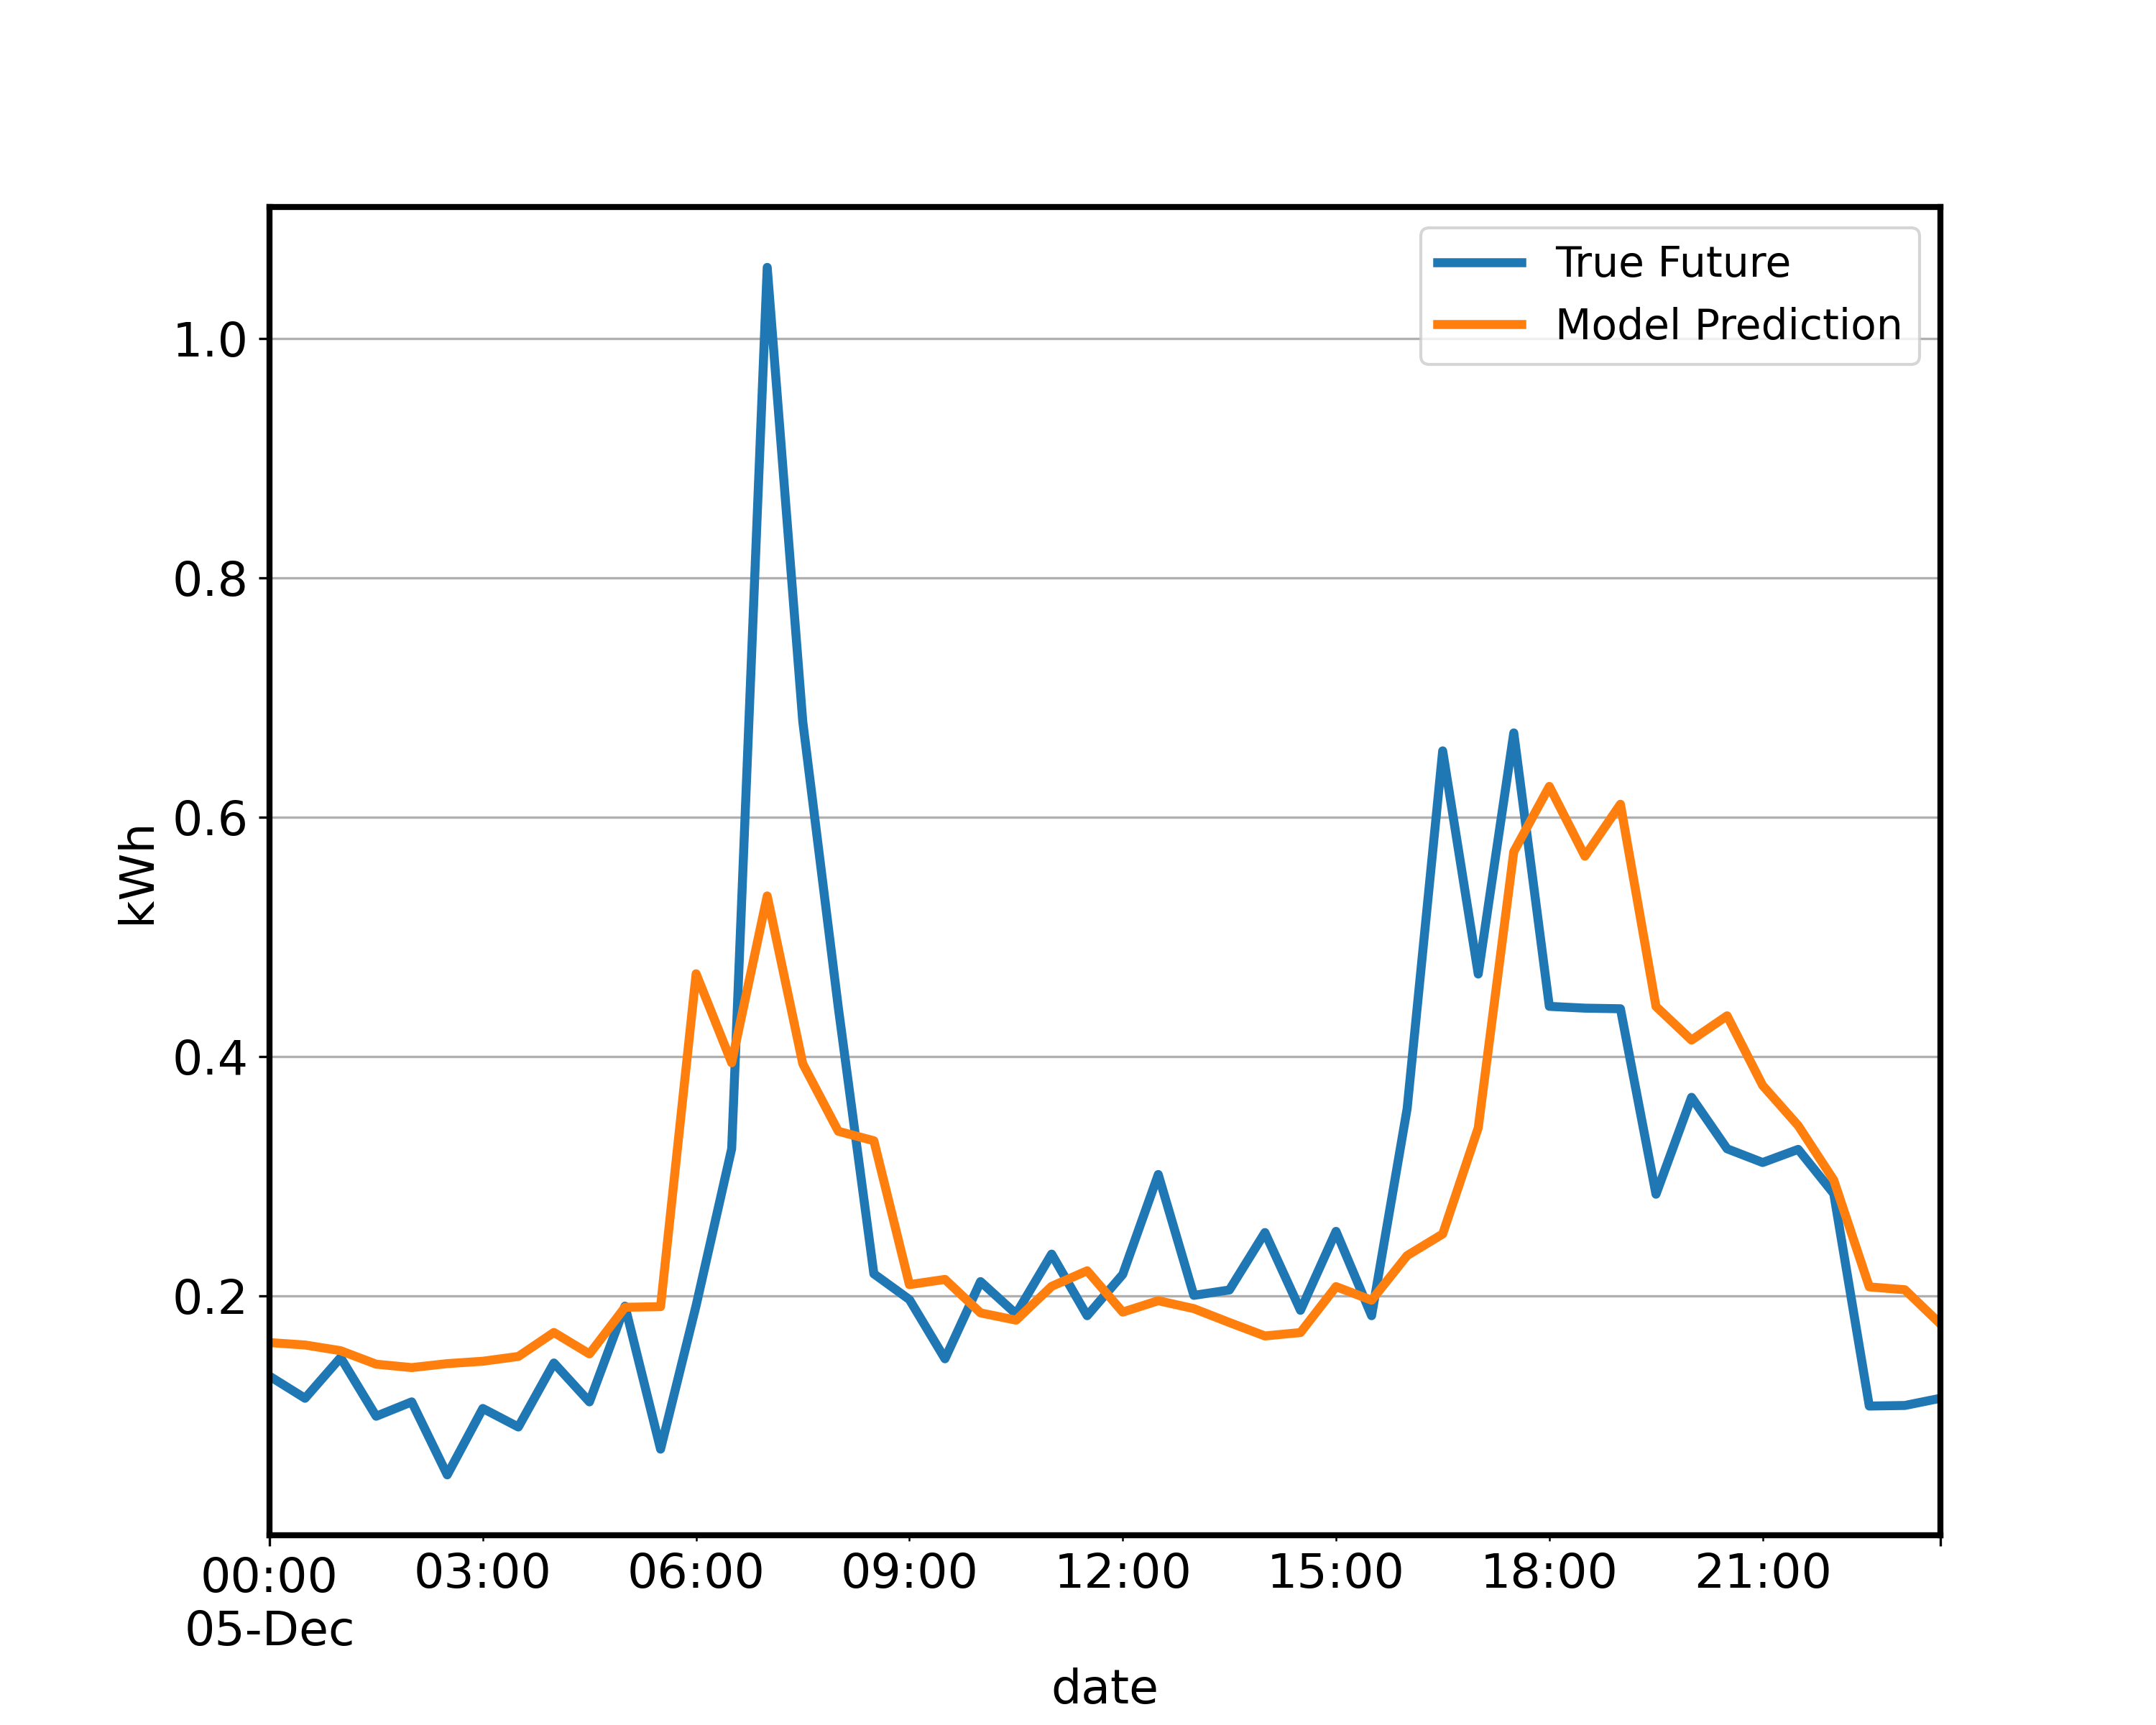
\includegraphics[width=1\linewidth]{mean_ID0x78a812ecd87a4b945e0d262aec41e0eb2b59fe1e_Day339_pred.png_1618425095.png}
		\caption{Model 4: ``Mean forecast''}
	\end{subfigure}	
	\begin{subfigure}{0.5\textwidth}
		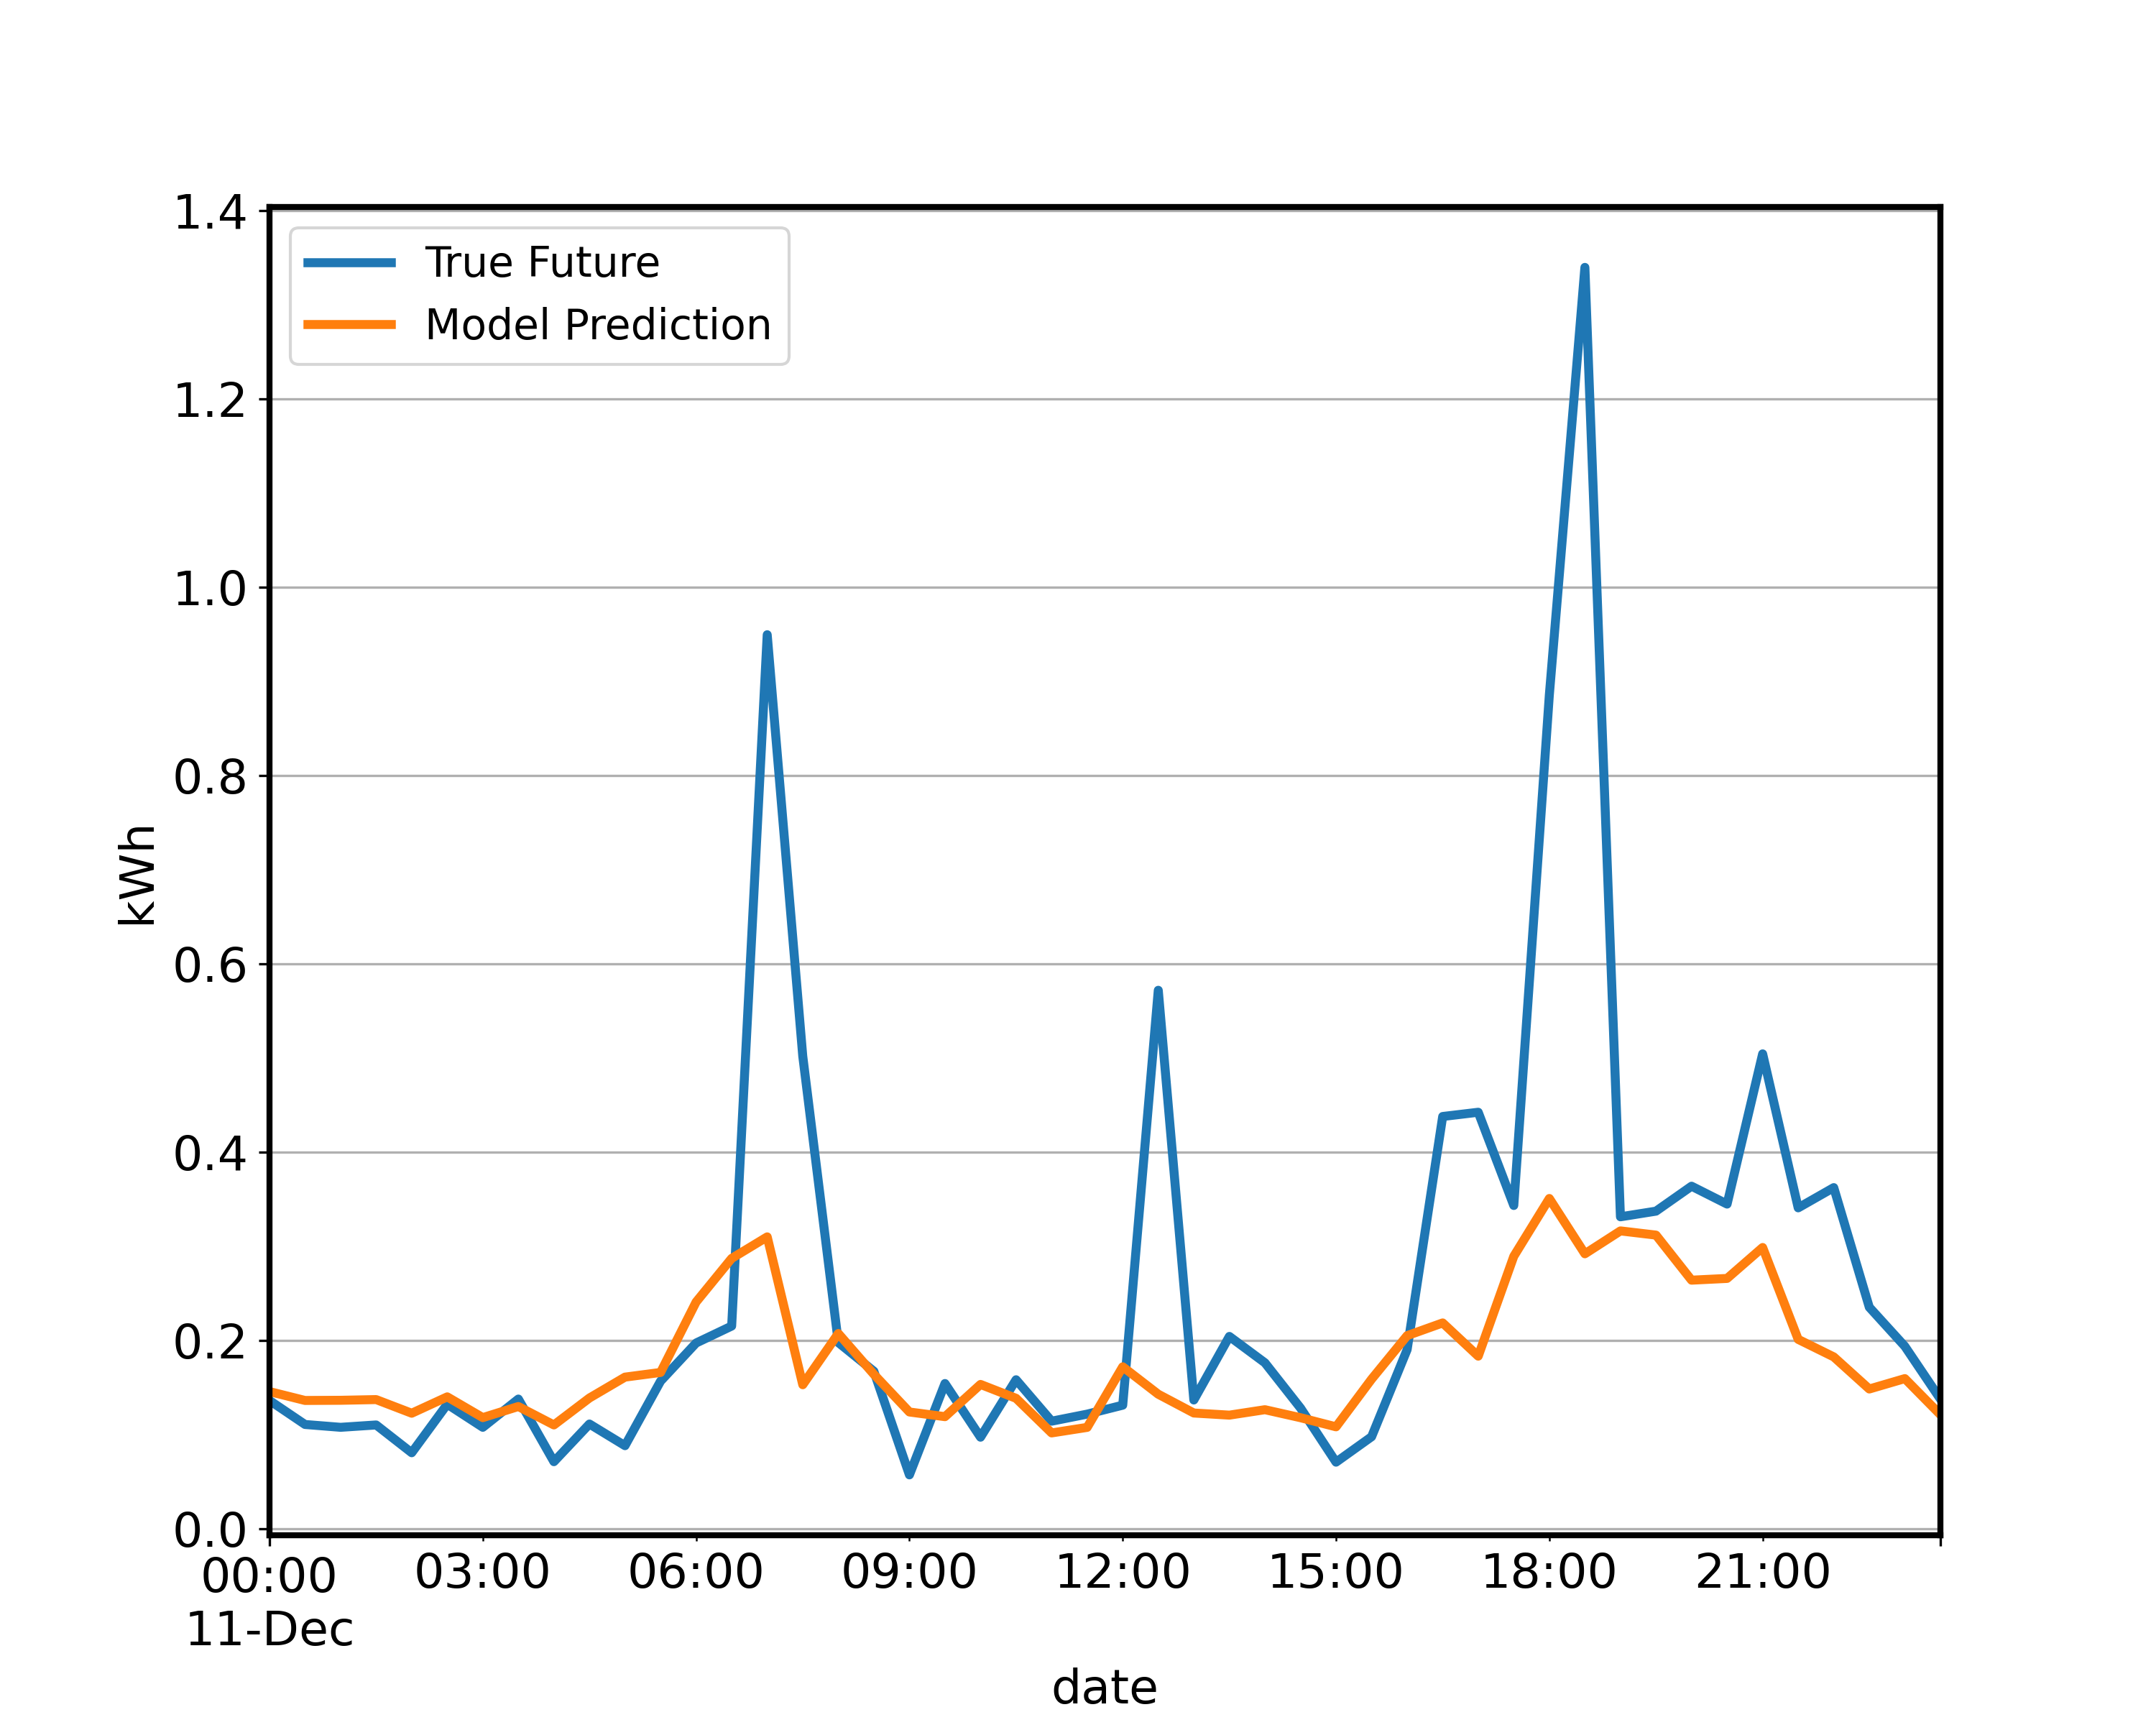
\includegraphics[width=1\linewidth]{MAPE_ID0x78a812ecd87a4b945e0d262aec41e0eb2b59fe1e_Day345_pred.png_1618425124.png}
		\caption{Model 5: ``MAPE forecast''}
	\end{subfigure}
	\caption{Daily predictions of two baseline models. (Blue: True / Orange: Prediction) }
	\label{fig:baseline models 4 and 5}
\end{figure}


In Table \ref{tab:summ_data_rel_performance} the overall performance of the baseline models on all $ 261 $ time series that contain a full year of measurements in the ``consumption.csv'', is given. The MAPE metric is not used because $ 99 $ series contain reference values of zero, which leads to a division by zero according to Eq. \ref{eq:MAPE}. Relative performance of a model on one serie is assessed by normalizing the error by division by the biggest error produced by one of the models. Therefore, the error of each serie is a value between one and zero and the model that performed worst will have an error of one. Finally, an average value is calculated over the different time series for each model. The closer the calculated value is to one, the more often this model performed worst with comparison to the other models. By applying this normalization, the NRMSE leads to the same result as RMSE. It is observed that the order of model performance based on the three metrics in Table \ref{tab:summ_data_rel_performance} over all the time series is: ``mean forecast'', ``MAPE forecast'', ``7 days ago forecast'', ``1 day ago forecast'' and finally ``closest day forecast''. From Table \ref{tab:summ_data_rel_performance} it is concluded that ``mean forecast'' is expected to give the best results on a randomly chosen time serie.

\begin{table}[ht]
	\centering
	\begin{tabular}{@{}l|ccccr@{}} \toprule
		\textbf{Error metric}	& \textbf{Closest day} & \textbf{$ 1 $ day} & \textbf{$ 7 $ days} & \textbf{mean} & \textbf{MAPE}\\\midrule
		Mean absolute error& \cellcolor{red!25}$0.950 $&$ 0.8298 $  & $0.8224 $ & \cellcolor{green!25}$ 0.7274 $ & $ 0.7918 $\\
		Mean squared error& \cellcolor{red!25}$0.8377 $&$ 0.7771 $  & $0.7363 $ & \cellcolor{green!25}$ 0.4996 $ & $ 0.6907 $\\
		Root mean square error& \cellcolor{red!25}$0.9084 $&$ 0.8621$  & $0.8426$ & \cellcolor{green!25}$ 0.6993$ & $ 0.8155$\\\bottomrule
	\end{tabular}
	\caption{Relative performance over all the $ 261 $ time series with a full year of measurements.}
	\label{tab:summ_data_rel_performance}
\end{table}


\section{Deep LSTM models}\label{s:Neural network models}
In this section deep LSTM models are presented in different variations. LSTM models are specialized in time series learning as discussed in Section \ref{s:LSTM}. The term ``deep'' refers to multiple LSTM layers that are stacked on top of each other. The goal of the developed models is to make a $ 24 $ hours ahead forcast of the electrical consumption of an individual household. First, practical considerations during the implementation of the models using Keras are discussed. Keras is a neural network library in Python which can be backend by Tensorflow which is an library for a number of various tasks in machine learning. This section covers the used inputs, batch size, choice between a stateless and stateful model, initialization, measures taken to avoid overfitting and the chosen error metrics. Next, the specific LSTM models developed are explained in Section \ref{s:LSTM_implementation}. Finally, the conducted parameter search is described in Section \ref{s:Parameter search}.

\subsection{Different practical considerations of the models in Keras}

\subsubsection{Inputs}\label{s:Inputs}
The inputs to theses models are normalized and similar as was suggested in papers \cite{loadforecastingmoor} and \cite{Kong2019}: 

\begin{itemize}
	\item Historic electrical consumption (min-max normalization)
	\item Average daily temperature (min-max normalization)
	\item Day of the week (one hot encoding)
	\item Time of the day (one hot encoding)
	\item Holiday (one hot encoding)
\end{itemize}

How far the model will look back into the history of electrical consumptions during a prediction, is determined by the lag value. This value corresponds to the amount of time steps that will be taken into account. The LSTM model in Keras expects a matrix $ \bm{X} $ as input with three dimensions: sample number, amount of time steps and amount of features. 
One sample of the $ \bm{X} $ matrix e.g. $ (1,lag\hspace{1.5mm}value, features) $, equals a 2D matix of dimensions  \textit{time steps} $ \times $ \textit{features}. Every column contains a different time serie that serves as input to the model. On the first column an amount of $ lag\hspace{1.5mm}value $ of previous consumption values is stored. The further down the rows of the first column, the closer time gets to the actual value that needs to be predicted. This is also the case for the temperature, but because temperature is only known on daily basis and the frequency of the values on the reference signal is one every thirty minutes, the temperature value is often the same in the second column of the 2D matrix. The values originating from the reference signal and daily average temperature serie are normalized by using a min-max normalization. Every value will now lay between zero and one.\\
In the next $ 7 $ columns of the 2D matrix, information is given about which day of the week it is. This is encoded making use of an one hot encoding. For every row one of the $ 7 $ columns which corresponds with the day of the week gets an one and the rest will be set to zero. Very similar the information about the time of the day is indicated. There are $ 48 $ columns and for every row only one column gets an one to indicate the time of the day. Finally, this is also done to indicate if it is a holiday. In total the input matrix $ \bm{X} $ has $ 59  $ columns which corresponds to the amount of features. Every sample of $ \bm{X} $ is used for a prediction of one time step of half an hour of the desired day. To make a 24 hours ahead prediction, the total $ 48 $ values are calculated recursively. Previous predictions are used in next ones by adding them to the history of electrical consumptions. The assumption is taken that the reference signal is available till the desired day. For example, if a prediction the electrical consumption of 19/12/2017 is desired, it is assumed that the reference signal is available till 18/12/2017 24:00.

\subsubsection{Batch size}
A batch size has to be specified in the Keras fit function. The batch size determines how many samples of $ \bm{X} $ are feeded to the model at once and their outputs compared with their reference to define an objective function. This objective function is used to calculate the gradients for weight updates. Because every sample of $ \bm{X} $ outputs one prediction value, the amount of samples of $ \bm{X} $ correspond to the amount of predictions made.\\

\subsubsection{Stateless versus Stateful}
Keras introduces a concept of stateless and stateful. As explained in Section \ref{s:Inputs} the input given to a LSTM model is a matrix with three dimensions: sample number, time steps, features. As explained in \cite{FneishMo} a stateless model interprets every sample of $ \bm{X} $ as if they have no relations with each other. A stateless model is not able to see that the different samples of $ \bm{X} $ originate from the same time series. Therefore, the hidden and memory states are reset when a new sample of $ \bm{X} $ is considered during model training and prediction. When the hidden states and memory states are reset, they are again initialized to zero vectors. If there is no relation between the different samples of $ \bm{X} $, it is logical to collect as much samples as possible and the input data is generated by moving a window every time one step further on the original time series as can be seen in Figure \ref{fig:stateless_input}.\\

A stateful model doesn't reset its hidden and memory states when considering a new sample of $ \bm{X} $. Because of this an additional condition is imposed to the input data that now, when all the samples of $ \bm{X} $ are glued behind each other, has to return the original times series sampled from. If this condition is not fulfilled, the hidden states and memory states would traverse a different serie than the original one. After one epoch during training the states are reset because the end of the original time serie has no connection with its start. During predictions the hidden and memory states are also preserved. Therefore, seeding of the model before prediction is possible as explained in Section \ref{s:Model3}.\\

The advantage of using a stateful model in comparison to a stateless one, is that during training and prediction more data can be presented to the hidden and memory states before they are reset. Therefore, the capability of the LSTM of long term remembering important features of the data, is more exploited. However, a practical disadvantage of using a stateful model is that Keras expects that the batch size chosen during training, equals the one during prediction. Each prediction uses one sample of input matrix $ \bm{X} $ to output one prediction value. This means that the batch size during training is forced to be equal to one. It was tried to circumvent this by first training on a model with chosen batch size and then transfer the learned model weights to a new, identical model with batch size one which would be used during the prediction. However, after testing it was found that the \textit{get\_weights()} and \textit{set\_weights()} commands in Keras didn't reproduce the same prediction results. It could only be used on the same model to set the weights to the ones, a chosen amount of epochs back during training. This is useful e.g. during the manual implementation of early stopping to restore the weights that performed best. In literature it was found that setting the weights on different models is possible when using the underlying Tensorflow library, but not in Keras. In addition, a stateful model expects that the training and validation sets are divisible by the batch size. To satisfy this condition samples of the input matrix can be thrown away. As will be seen in Section \ref{s:Model3}, it was chosen to set the batch size of the developed stateful model 3 equal to one which is called ``online learning'' in literature. Both the previous conditions are then fulfilled.\\


To avoid these issues, it was first experimented with using a batch size during training that was bigger than one and then rebuilding the model with a batch size of one. The latter model would then be used during prediction. The trained weights of the first model where transferred to the second model. However, after testing it was found that the \textit{get\_weights()} and \textit{set\_weights()} commands in Keras didn't reproduce the same prediction results when used on different models. It could only be used on the same model to set the weights to the ones a chosen amount of epochs back during training. This is useful e.g. during the manual implementation of early stopping to restore the weights that performed best. 

It was chosen to set the batch size issues for a stateful model by setting the batch size 

\begin{figure}[h]
	\centering
	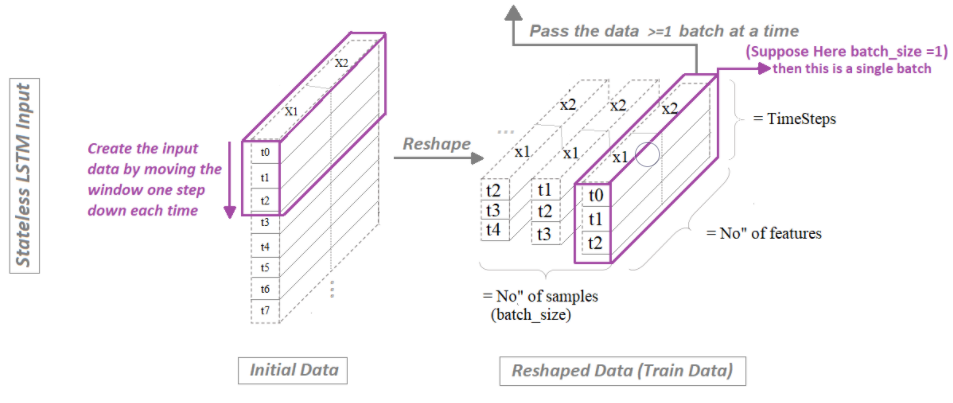
\includegraphics[width=1.2\textwidth]{stateless_input.png}
	\caption{The generation of inputs for a stateless model. (source: \cite{FneishMo})}
	\label{fig:stateless_input}
\end{figure}

\begin{figure}[h]
	\centering
	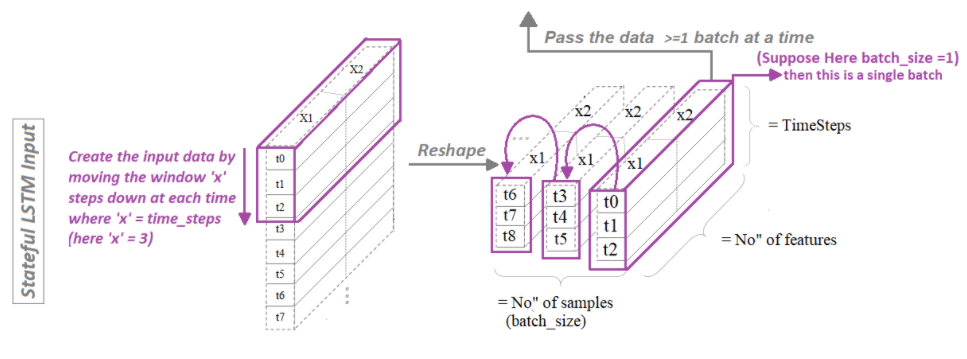
\includegraphics[width=1.2\textwidth]{stateful_input.png}
	\caption{The generation of inputs for a stateful model. (source: \cite{FneishMo})}
	\label{fig:stateful_input}
\end{figure}

\subsubsection{Initialization}
The LSTM equations in Section \ref{s:LSTM} show four weight matrices $ \bm{W} $ with an index \textit{H} and four weight matrices with an index \textit{X}. These are respectively the recurrent and kernel weights and they are both initialized in a different way. A recurrent weight matrix is initialized using an orthogonal initialization and the kernel weight matrix uses a glorot uniform initialization. Both methods make use of random sampling of a distribution  during the generation of the initial values. The biases $ \bm{b} $, memory states $ \bm{c}_t $ and hidden states $ \bm{H}_t $ of the LSTM equations are all initialized by arrays filled with zeros.\\

\subsubsection{Overfitting avoidance in Keras}
Different ways to avoid overfitting can be applied in Keras::
\begin{itemize}
	\item Early Stopping
	\item Dropout and recurrent dropout in the LSTM layer
	\item Dropout in the Dense layers
	\item $ l2 $ regularization on the kernel weights, recurrent weights, bias and activity.
\end{itemize}


\subsubsection{Error metrics}
The  MAE metric is used to evaluate the prediction performance on the validation set during the parameter search in Section \ref{s:Parameter search}. During training the MSE is used in the objective function which is used to derive weight updates.


\subsection{Deep LSTM}\label{s:LSTM_implementation}
\begin{figure}[ht]
	\centering
	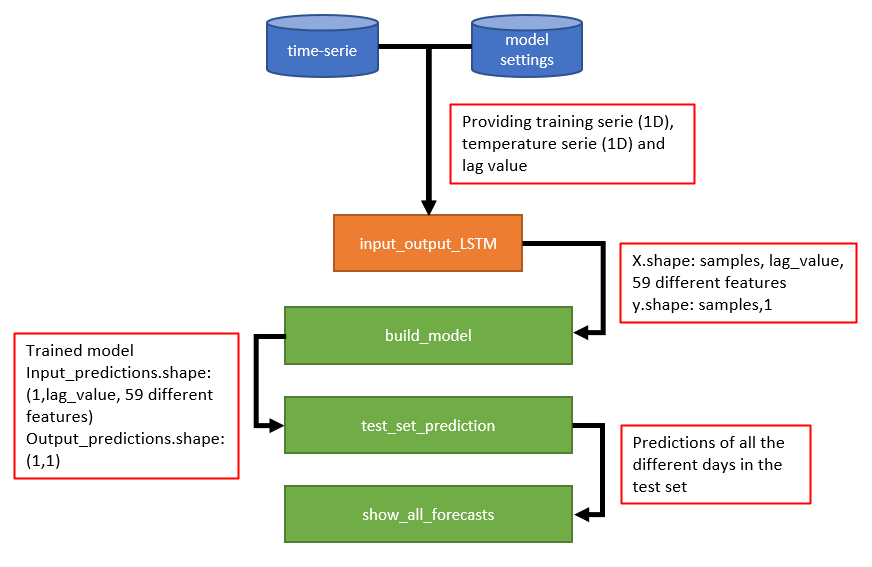
\includegraphics[width=1.2\textwidth]{flow_code.png}
	\caption{The flow of functions that are executed in order during the prediction process with LSTM models.}
	\label{fig:model1}
\end{figure}


First, the input data of the LSTM is calculated in \textit{input\_output\_LSTM}. This is done before training using the GPU that is listed in Table \ref{tab:CPU}. The inputs that are used are discussed in Section \ref{s:Inputs}. Next, the models are build. Three different models will be shown further from which the first two are stateless models and the third is a stateful model. For the stateless models it is possible to shuffle the input data. When it is desired that before splitting the inputs of the LSTM in a training and validation set, the data is shuffled and not just the last part is taken as validation set, shuffling should be done manually before the inputs are assigned to the Keras fit function according to Deeplizard's blog page. During prediction, every model will predict one value at at time as was proposed as a good methodology in \cite{ANNRNN}. This means that $ 48 $ predictions are needed for a $ 24 $ hours ahead prediction. Each model makes use of early stopping on a validation set to avoid overfitting. The models can have multiple LSTM layers on top of each other. The hidden state vector $ \bm{H}_{j} $ serves then as input instead of $ \bm{X}_{k} $ for the layer above. The specific parameters and layout that is chosen for each of the three models is discussed in Section \ref{s:Parameter search}.

\subsubsection{Model 1: Stateless with no flatten layer}\label{s:Model1}

\begin{figure}[h]
	\centering
	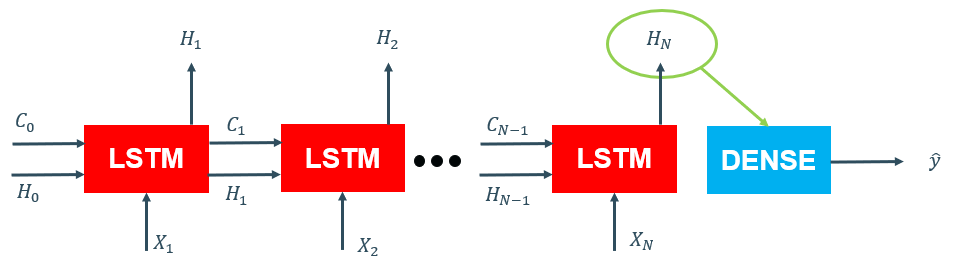
\includegraphics[width=1.2\textwidth]{model1.png}
	\caption{Model 1 - stateless model with as input a subserie of N time steps and $ \bm{C}_{i} \in \mathbb{R}^{m} $, $ \bm{H}_{j} \in \mathbb{R}^{n} $, $ \bm{X}_{k} \in \mathbb{R}^{59} $, $ \hat{y} \in \mathbb{R}^{1} $.}
	\label{fig:model1}
\end{figure}

One sample of the input matrix $ \bm{X} $ consists of $ N $ timesteps which are feeded to the LSTM layer as is shown in Figure \ref{fig:model1}. $ N $ equals to the chosen lag value. When the final LSTM block is reached the output of this block will be translated to a single prediction value by a conventional layer of hidden neurons (Dense layer). The subseries are created by shifting the window one time step further as is explained in Section \ref{s:Inputs}. Because Model 1 is stateless $ \bm{C}_{0} $ and $ \bm{H}_{0} $ will be initialized as zero vectors. Although that Figure \ref{fig:model1} gives the impression that there are multiple LSTM blocks, this only serves as a visual interpretation. There is actually only one LSTM block that is reused for every $ \bm{X}_{k} $. This means that when the same amount of layers and hidden recurrent states are chosen, all the three models will have the same amount of trainable parameters. 


\subsection{Model 2: Stateless with flatten layer}\label{s:Model2}

\begin{figure}[ht]
	\centering
	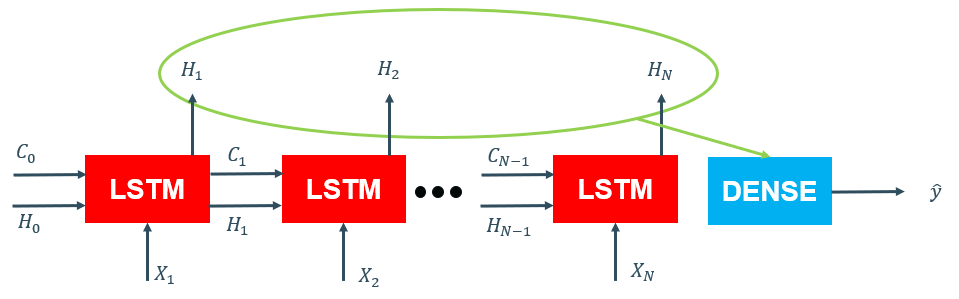
\includegraphics[width=1.2\textwidth]{model2.png}
	\caption{Model 2 - stateless model with as input a serie of N time steps and $ \bm{C}_{i} \in \mathbb{R}^{m} $, $ \bm{H}_{j} \in \mathbb{R}^{n} $, $ \bm{X}_{k} \in \mathbb{R}^{59} $, $ \hat{y} \in \mathbb{R}^{1} $.}
	\label{fig:model2}
\end{figure}

Additionally to the output of the last LSTM block also the previous outputs of the LSTM blocks are inputs to the dense layer. This model corresponds to the model depicted in \cite{Kong2019}.

\subsection{Model 3: Stateful}\label{s:Model3}
\begin{figure}[ht]
	\centering
	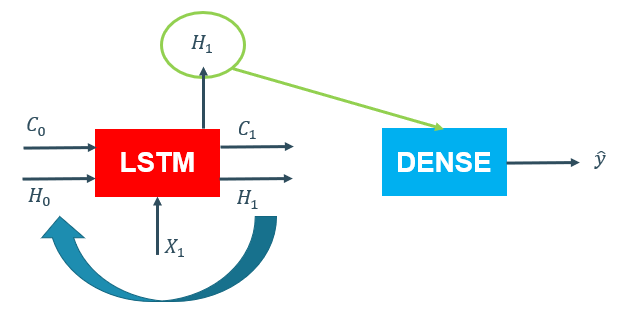
\includegraphics[width=0.8\textwidth]{model3.png}
	\caption{Model 3 - stateful model that connects single LSTM blocks and $ \bm{C}_{i} \in \mathbb{R}^{m} $, $ \bm{H}_{j} \in \mathbb{R}^{n} $, $ \bm{X}_{k} \in \mathbb{R}^{59} $, $ \hat{y} \in \mathbb{R}^{1} $.}
	\label{fig:model3}
\end{figure}

Where the previous two models only go through a subserie before making a prediction, this model sees the whole original time serie when making predictions. This is possible because the model looks one by one at each sample of the original time serie. For example $ \bm{X}_{1} $ is feeded to the model and $ C_{1} $ and $ H_{1} $ come out.  $ C_{1} $ and $ H_{1} $ are now again set as $ C_{0} $ and $ H_{0} $ when the next sample $ \bm{X}_{2}  $ is used. This means that the model glues every subserie of one value together, which recreates the original serie. The shape of $ \bm{X} $ is now $ (15500, 1, 59) $, so each sample now is not a 2D matrix but an array. After training and before prediction of the test set or validation set, it is important that the memory states $ \bm{C}_{i} $  and hidden states $ \bm{H}_{j} $ are set ``right'' for prediction. Therefore, the model is first seeded, which means that first all the inputs before the desired day are shown to the model. When the model then reaches the desired day, it had the chance to collect important information in the memory states and the hidden states that can be used during the prediction. During the consecutive predicting of a 24 hours ahead forecast, the model only uses previous predictions as input in comparison to Model 1 and 2, who use a serie as input of each prediction with at the end the previous predicted values.

\subsection{Parameter search}\label{s:Parameter search}
This section will show that the different LSTM models are dependent on the choice of good parameters to perform well. During a parameter search different values for the parameters are tried and the values that give the best results, are retained. Because it is not straightforward what the influence of one parameter exactly is on the model, all the different parameters are assumed to depend on each other. If all the different parameters are varied simultaneously the calculation load will rapidly blow up. To deal with this, the parameter search is conducted in three stages. The cost of this reduction in calculation load will be that dependencies between parameters are neglected. During the parameter search every combination is repeated three times to reduce the influence of the random initialization of the weights in the weight matrices. The error value that is used to decide if a combination of values behaves better or worse, is based on the MAE on the $ 10 $ last days of November of three runs. This validation set is used for all three models on all three series. Only $ 10 $ days are chosen to reduce the calculation load. An advantage of using this validation set in comparison with cross-validation is that it can be used for all models. Cross-validation for Model 3, is not possible because it would cause interruptions in time. Inspiration for the values tried during the parameter search is partly based on \cite{Shi2018}.

\begin{itemize}
	\item Stage1: different model layouts are tried (calculation time $ \approx $ $ 10 $ hours)
	\item Stage 2: the most complex model is chosen and regulation is added (calculation time $ \approx $ $ 6\times4 $ hours)
	\item Stage 3: after comparing the previous stages, the best is chosen and the learning rate is more precisely tuned (calculation time $ \approx $ $7$ hours)
\end{itemize}

\begin{table}[ht]
	\centering
	\begin{tabular}{@{}l|r@{}} \toprule
		\textbf{Parameter}	& \textbf{Values}\\\midrule
		Hidden states &  $ [20,50] $\\
		LSTM layers & $ [1,3] $\\
		Neurons dense layer & $ [50] $\\
		Dense layers & $ [1] $\\
		Lag value & $ [48,96] $\\
		Number epochs & $ [2] $\\
		Batch size & $ [48] $\\
		Learning rates & $[ 10^{-4} $,$ 10^{-3} $,$ 10^{-2} ]$\\
		Shuffle & $ [True] $\\
		Repeat & $ [3] $\\\bottomrule
	\end{tabular}
	\caption{Parameters used during phase 1 for the two stateless models.}
	\label{tab:para_phase1}
\end{table}

The values tried for the different parameters are displayed in Table \ref{tab:para_phase1}. A total of $ 24 $ combinations is tried during phase one and each combination is run $ 3 $ times. The batch size chosen is only one number to make a fair comparison between the different settings with respect to the amount of weight updates that will be performed. With a batch size of $ 48 $, there are around $ \frac{15500}{48}\approx 320 $ weight updates per epoch and $ 640 $ in total. One LSTM layer is compared with three LSTM layers on top of each other in order to see a clear difference in the influence of the amount of LSTM layers used. Only two epochs are considered to reduce the calculation load and therefore early stopping is not used.\\

Changes to the parameters in Table \ref{tab:para_phase1} are made for model $ 3 $. In model $ 3 $ a batch size of one, a lag value of one and shuffling ``False'' are used. A batch size of one is chosen because then the prerequisites for a stateful model as discussed in Section \ref{s:Model3}, is fulfilled.\\

In phase two, the assumption is made that a more complex model will be able to better capture the non-linear relations in the data and regulation is added to avoid overfitting behaviour. The learning rate that was part of combination of parameter values that performed best during phase one, is selected together with the lag value. During phase two the amount of hidden states is taken equal to $ 50 $ and the amount of LSTM layers to $ 3 $. The regulation that is shown in Table \ref{tab:regulation}, is always added one at a time. The synergy between different regularization methods is thus neglected. 

\begin{table}[ht]
	\centering
	\begin{tabular}{@{}l|r@{}} \toprule
		\textbf{Kind of regularization} & 	\textbf{Kind of dropout}\\\midrule
		regularizer on input weight matrix LSTM 	& dropout inputs LSTM\\\hline
		regularizer on recurrent weight matrix LSTM & dropout recurrent states\\\hline
		regularizer on DENSE layer & dropout dense layer\\\hline
		$[ 10^{-2} $,$ 10^{-3} $,$ 10^{-4}$, $ 10^{-5} ]$ & $[ 0.2 $,$ 0.3 $,$ 0.4$, $ 0.5 ]$\\\bottomrule
\end{tabular}
\caption{Different regularization added during phase 2.}
\label{tab:regulation}
\end{table}


When l2-norm regularization is added to a weight matrix, the size of the weight using the l2-norm is added in the objective function. This means that big weight values are seen as an artificial error and the model tries to keep the weights small. The regularization parameter defines the ratio between the model focussing on the error with the reference signal and the size of the weights. Setting a big regularization parameter will give a model that becomes less ``expressive''. Therefore, the regularization parameter will contribute in the avoidance of overfitting.\\ 
The dropout layer that is used after the LSTM layer and after the Dense layer sets a rate of its inputs to zero. Similar, the dropout and recurrent dropout parameters in the LSTM layer drop respectively a rate of its inputs $ \bm{X}_{k} $ and $ \bm{H}_{j} $ to zero. The dropout rate values that are chosen are chosen between $ 0.2 $ and $ 0.5 $ as is advised in \cite{Mele1993}.\\

As will be further shown and as was found in \cite{Greff2017}, the learning rate is a very important parameter that has to be tuned correctly to enhance the model performance. Therefore a bigger range of learning rates is tried for the model that performed best after stage one and two of the parameter search. Afterwards, the learning rate which leads to the the smallest error is selected. The different learning rates that are tried are $ 10^{-2} $, $ 5\times10^{-3} $, $ 2\times10^{-3} $, $ 10^{-3} $, $ 10^{-4} $ and $ 10^{-5} $. \\

In order to speed up the calculations, multithreading is implemented to calculate separate runs in different threads. It was found that one thread takes considerably longer than when the full CPU is used to calculate the same run, but still a time gain is obtained in a total of $ 4 $ runs.\\

The importance of setting good parameters is stressed by the fact that for certain parameters the loss during training becomes ``not a number''. This is because the model becomes unstable and gets a very big loss which eventually becomes a nan. When this occurs the model is tried again with different initialization of the weights, which often solves the problem or a nan value is included as error. 


\subsubsection{Model 1: Stateless with no flatten layer}

\textbf{Phase1:}\\
Table \ref{tab:relative_performance_parameters_phase_one_model_one} shows the parameter search using the parameters listed in Table \ref{tab:para_phase1}. The search was ran on a local machine (see Table \ref{tab:CPU}) for $ 9 $ hours and $ 48 $ minutes. It is clear from Table \ref{tab:relative_performance_parameters_phase_one_model_one} that when the learning rate is varied this has the most impact on the average performance of the model. This result corresponds with paper \cite{Greff2017} where it was concluded that this parameter is the most important when tuning a LSTM. Next, it can be seen that the lag value of $ 96 $ time steps didn't lead to much more improvement with respect to looking at $ 48 $ historic time steps during every prediction. A reason for this can be that the day, two days ago, is not very representative for the desired day. It can be argued that the desired day a week ago would add more value, because this better captures the human weekly routine. In comparison Model $ 3 $ traverses the whole historic signal before making predictions. It is therefore expected that that model better captures the weekly routine.\\
An unexpected result that was found is that less LSTM units and only one LSTM layer in the case of Serie 1 gives raise to a lower MAE. The reason for this could be the presence of overfitting when using a more complex model. Table \ref{tab:best_performing_para_phase1} gives the combination of settings that performed best during phase one. In the next phase of the parameter search, regulation is added and compared with the results obtained during phase one of the parameter search. \\

\begin{table}[ht]
	\centering
	\begin{tabular}{@{}l||c|ccc@{}} \toprule
		\multicolumn{5}{c}{Model 1: Stateless (no flatten layer)}\\\midrule\midrule
		\textbf{Chosen parameter}	& \textbf{Value} & \textbf{Serie $ 1 $} & \textbf{Serie $ 2 $} & \textbf{Serie $ 3 $}\\\midrule
		Units LSTM & $ 20 $ & $12.08 $		&$ 1.24 $  & $1.48 $\\
		 		   & $ 50 $ & 		  		&		   & 		\\\hline
		layers LSTM & $ 1 $ & $9.82 $		&		   & 		\\
				    & $ 3 $ & 	      		&$ 4.26 $  & $5.80$\\\hline
		Lag value & $ 48 $ & $4.25 $ 		&		   & $0.390$\\
				  & $ 96 $ &          		&$ 2.06 $  & 		\\\hline
		Learning rate & $ 10^{-2} $ &       &		   & 		\\
					& $  10^{-3} $ &$0.0594 $&$ 17.2$  & $10.6$\\
					& $  10^{-4} $ &$8.74 $&$ 25.0$    & $12.2$\\\bottomrule
			
	\end{tabular}
	\caption{Each value in this table shows the average error when the value of a chosen parameter was used, normalized by the biggest error of the possible values and finally subtracted by one. Therefore, each value shows a percentage of improvement with respect to the worst possible value for a chosen parameter for each serie during phase $ 1 $ of the parameter search. For example: when $ 20 $ LSTM units are chosen, this on average gave a $ 12.08\% $ lower MAE.}
	\label{tab:relative_performance_parameters_phase_one_model_one}
\end{table}


\begin{table}[ht]
	\centering
	\begin{tabular}{@{}l|ccc@{}} \toprule
		\multicolumn{4}{c}{Model 1: Stateless (no flatten layer)}\\\midrule\midrule
		\textbf{Parameters}	& \textbf{Serie $ 1 $} & \textbf{Serie $ 2 $} & \textbf{Serie $ 3 $}\\\midrule
		Units LSTM & $20 $&$ 50 $  & $20 $\\
		layers LSTM & $1 $&$ 3 $  & $3$\\
		Lag value & $96 $&$ 96$  & $48$\\
		Learning rate & $0.01 $&$ 0.0001$  & $0.0001$\\\hline
		MAE error 1   & $ 0.133 $ & $ 0.0426 $ & $ 0.100 $\\
		MAE error 2   & $ 0.135 $ & $ 0.0433 $ & $ 0.100 $\\
		MAE error 3   & $ 0.138 $ & $ 0.0428 $ & $ 0.101 $\\\bottomrule
	\end{tabular}
	\caption{The values of the parameters that performed best for the three time series during phase $ 1 $ using model $ 1 $ based on the smallest sum of MAE errors during three runs.}
	\label{tab:best_performing_para_phase1}
\end{table}


\textbf{Phase 2}\\
In this section the learning rate and the lag value of the best performing model are combined with the most complex model with regulation. With most complex model, it is meant that $ 50 $ LSTM units and $ 3 $ LSTM layers are used. A sensitivity analysis is done to look which regulation has the most effect. Finally, the results of phase two are compared with the best results of phase one. Note, that using this approach assumes that adding regulation can nullify the use of a too complex model. When LSTM regularization is added this done the same on each LSTM layer.


\begin{figure}[h!]
	\centering
	\begin{subfigure}{0.49\linewidth}
		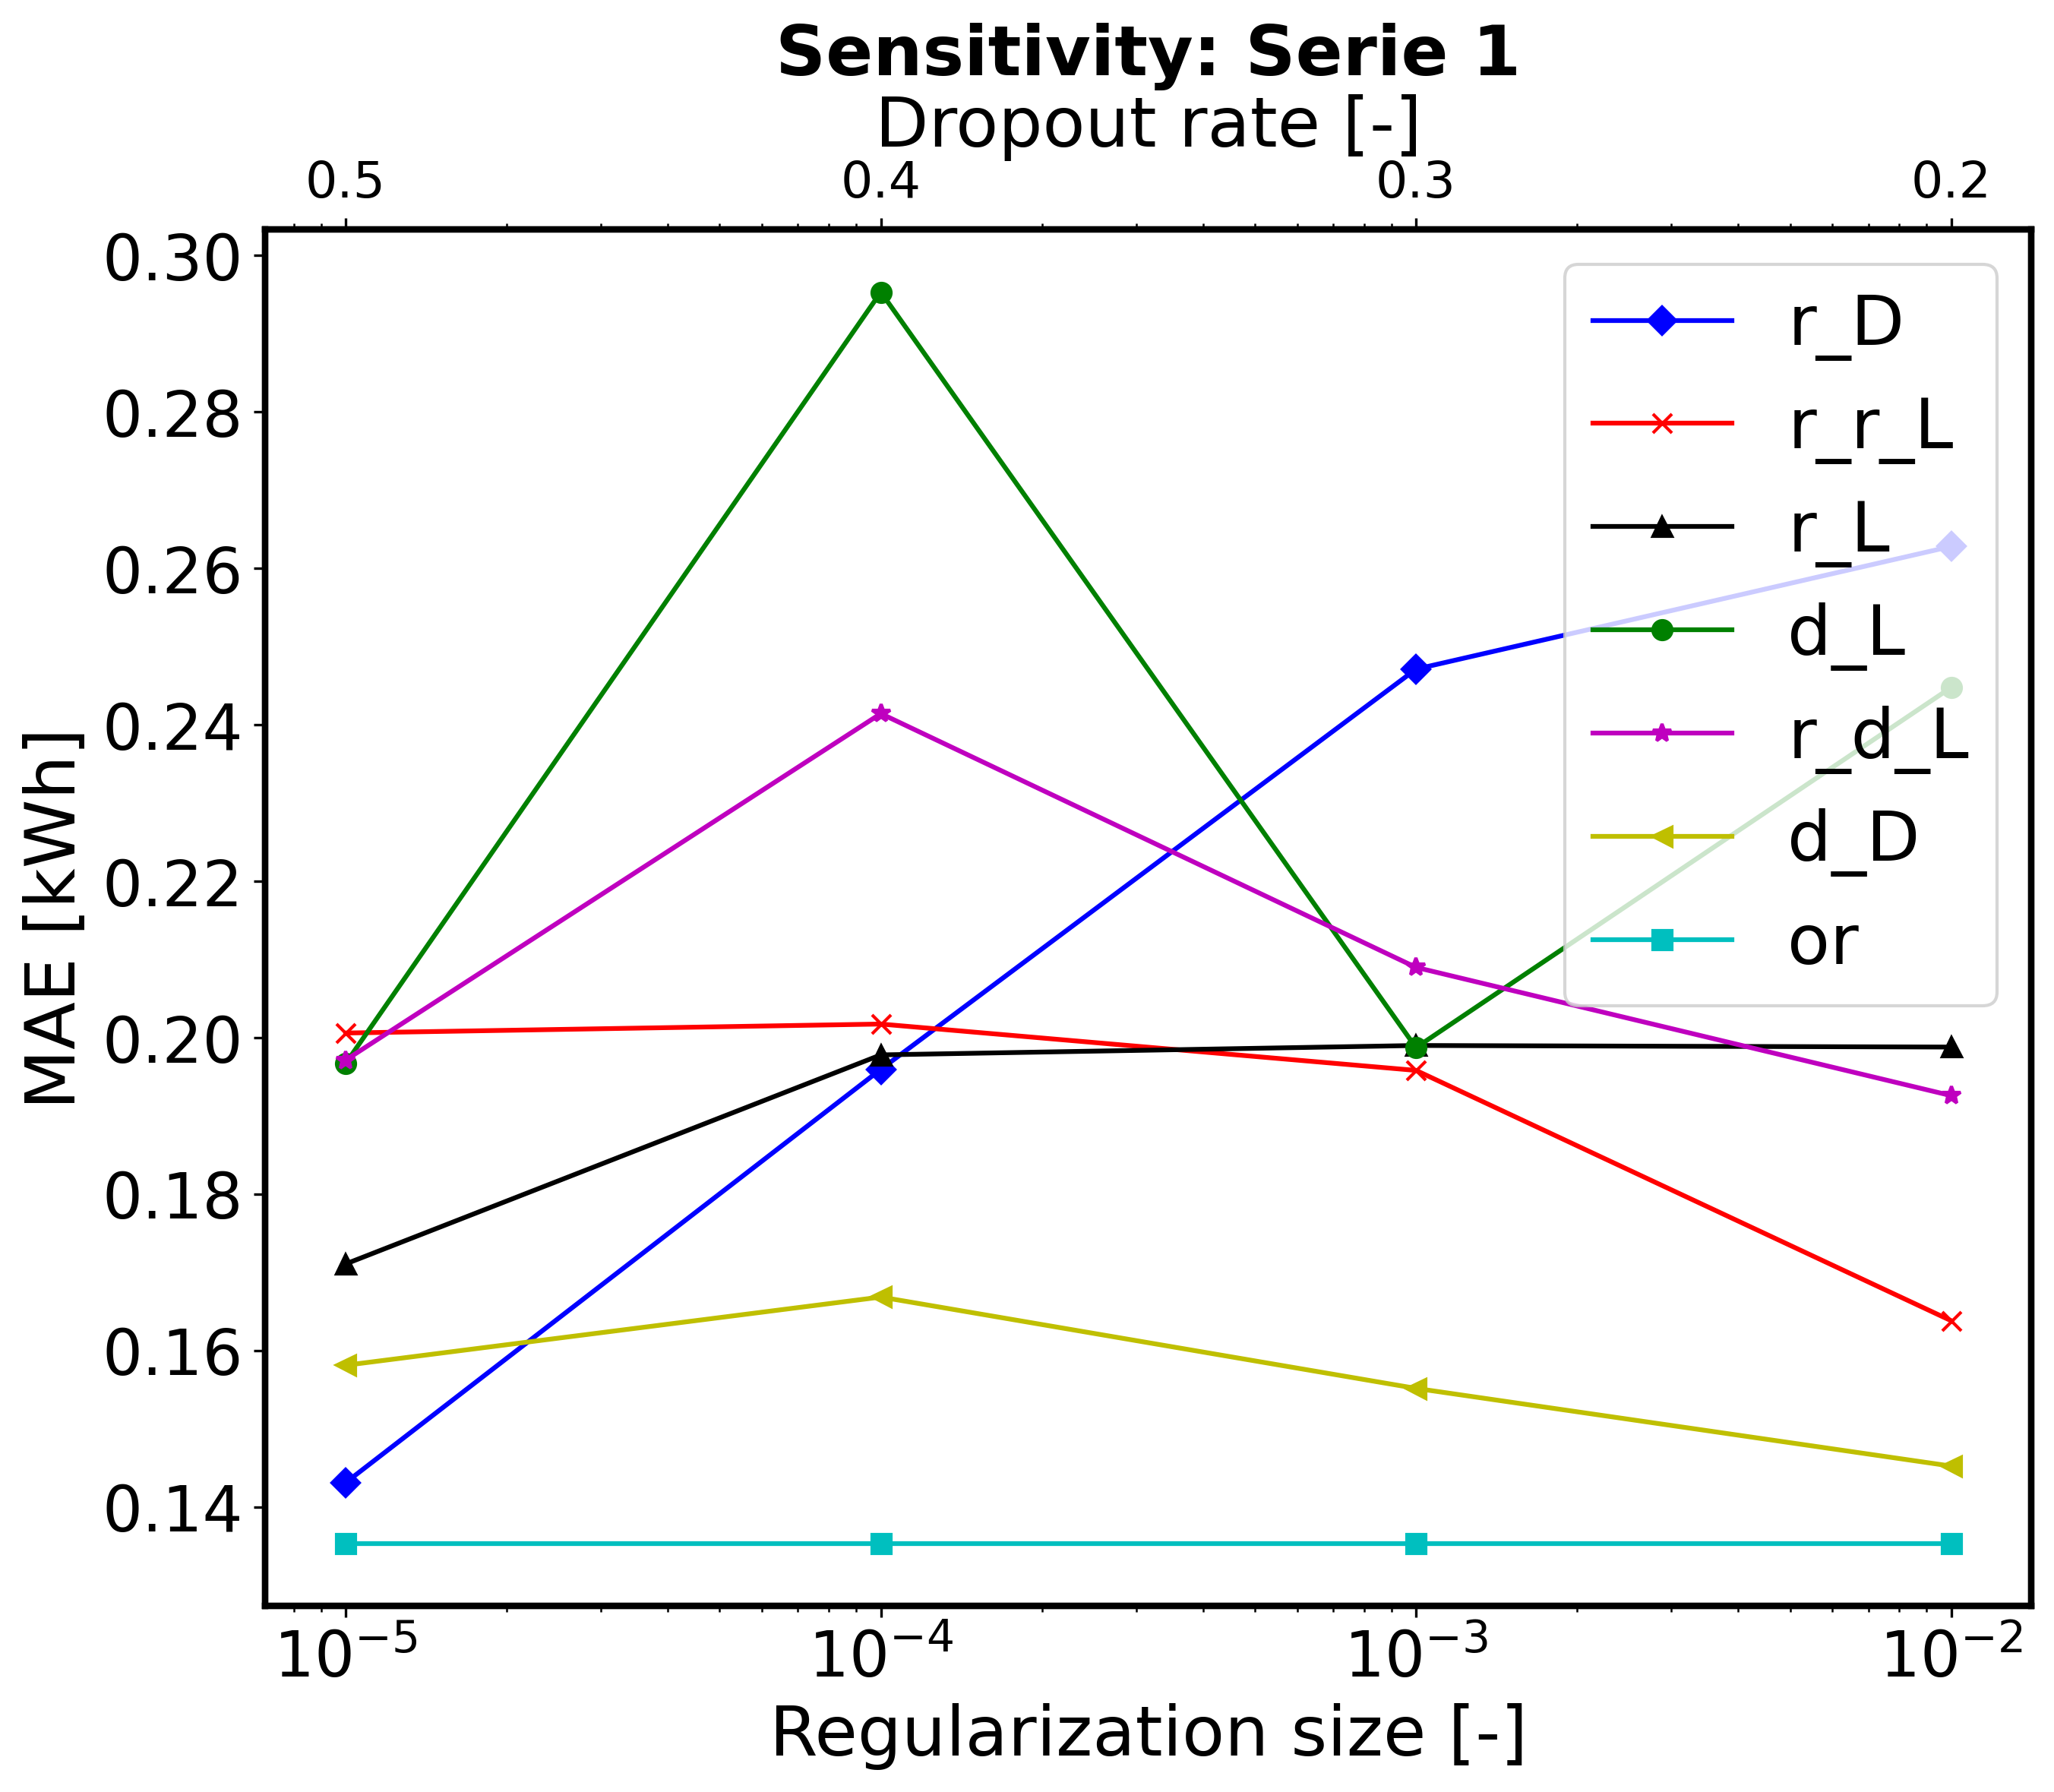
\includegraphics[width=1\linewidth]{serie1_model1.png}
		\caption{Model 1}
	\end{subfigure}	
	\begin{subfigure}{0.49\linewidth}
		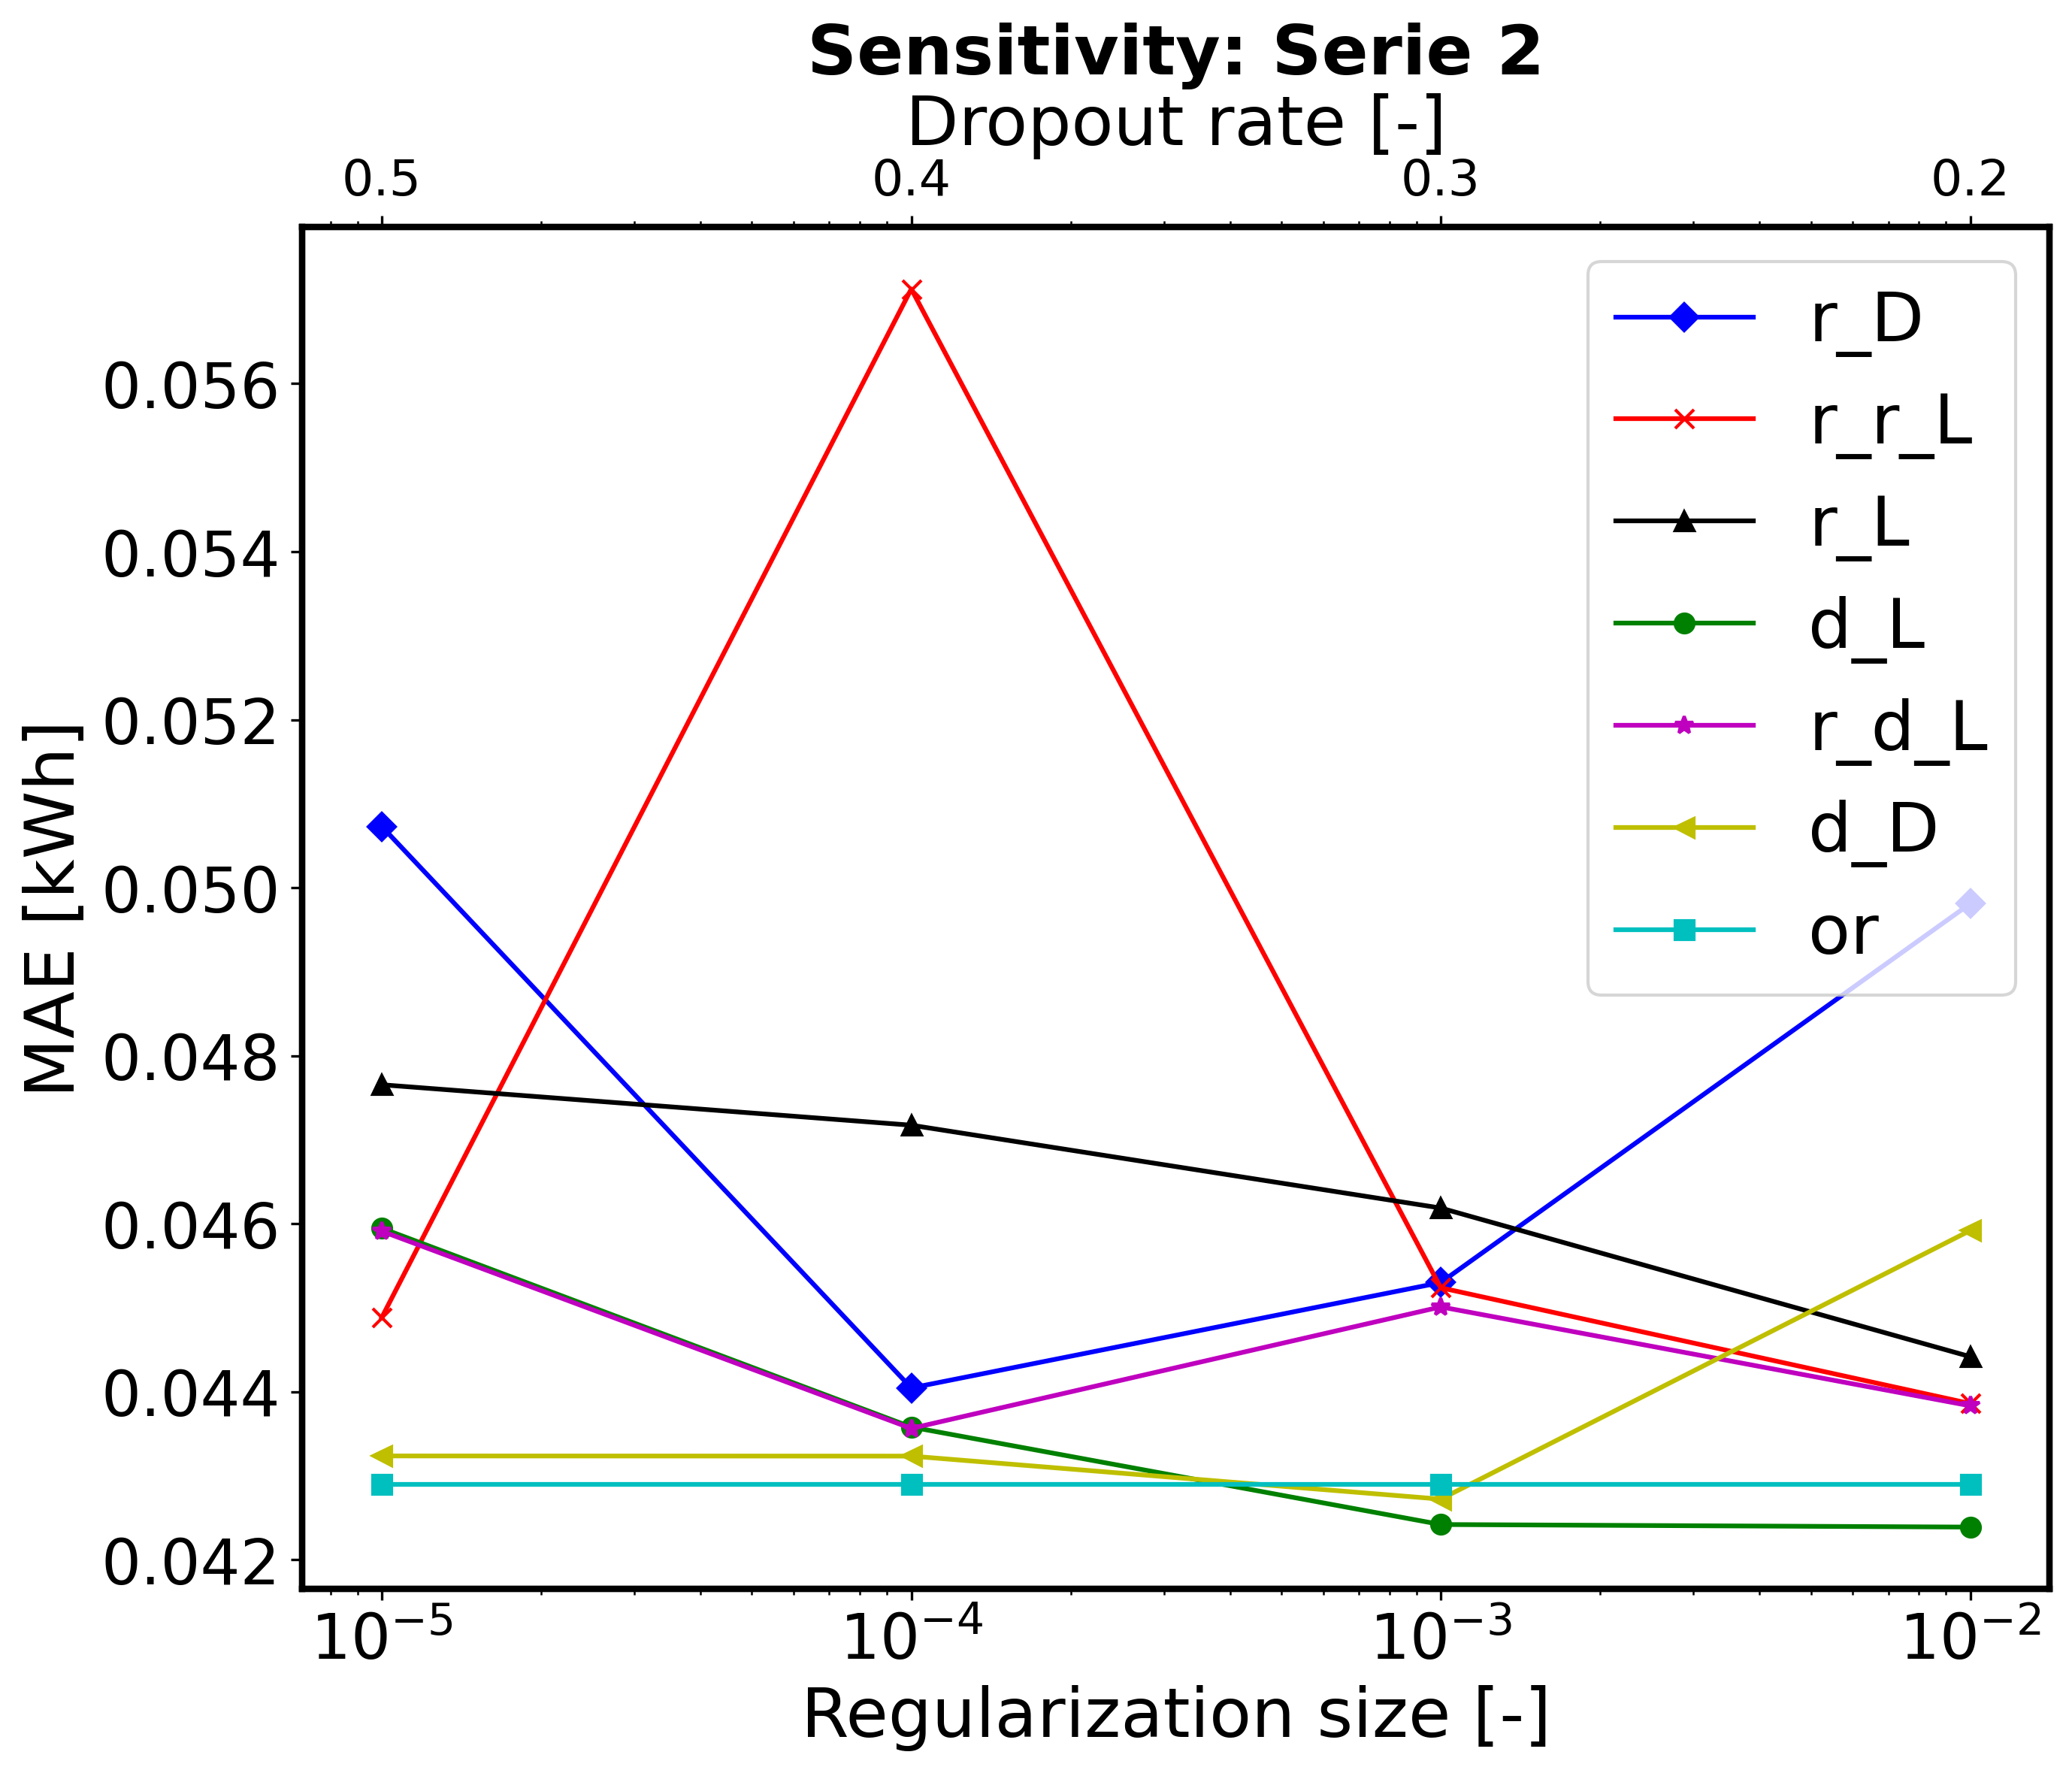
\includegraphics[width=1\linewidth]{serie2_model1.png}
		\caption{Model 1}
	\end{subfigure}
\begin{subfigure}{0.5\linewidth}
	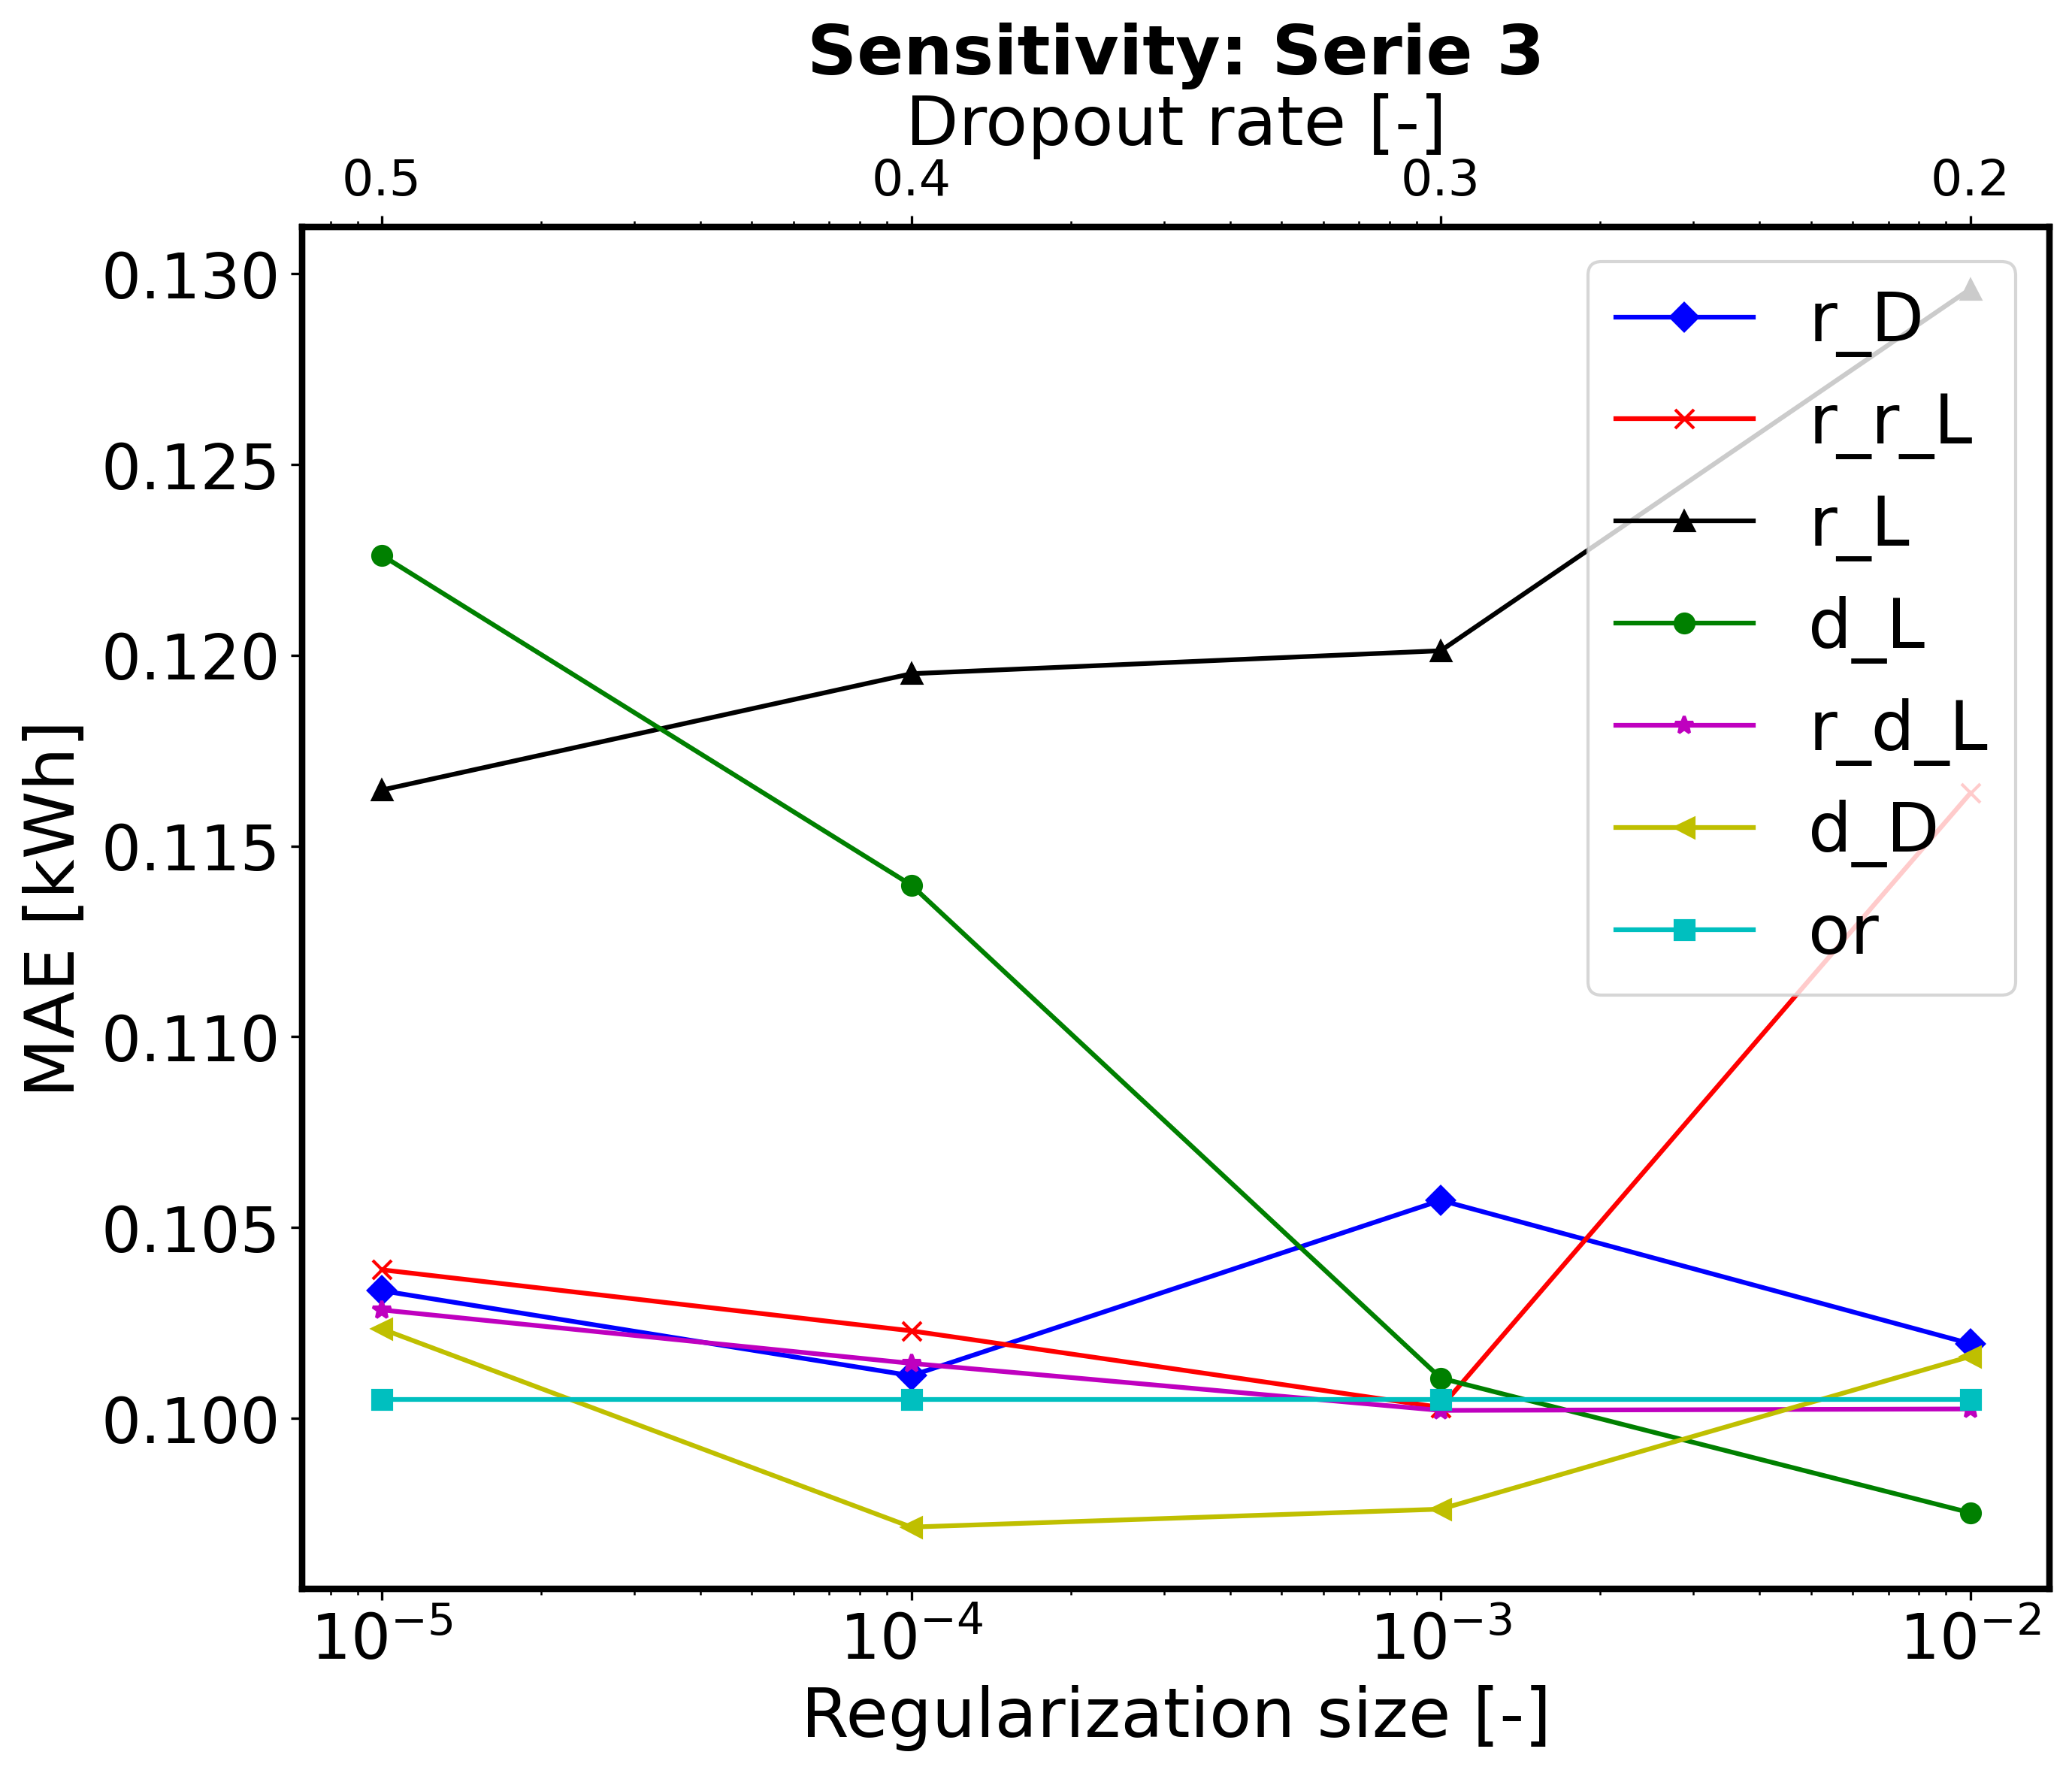
\includegraphics[width=1\linewidth]{serie3_model1.png}
	\caption{Model 1}
\end{subfigure}
	\caption{Results of the sensitivity analysis on the size of regulation parameter and the dropout rate with respect to the mean absolute error.(Legend: \textit{r\_D}: regularization size of weights DENSE layer,  \textit{r\_r\_L}: regularization size of recurrent weight of LSTM, \textit{r\_L}: regularization size of input weights of LSTM, \textit{d\_L}: dropout rate of input states LSTM, \textit{r\_d\_L}: dropout rate of recurrent states LSTM, \textit{d\_D}: dropout rate of DENSE layer, \textit{or}: best performing serie from phase one)}
	\label{fig:sensitivity_model1}
\end{figure}

From Figure \ref{fig:sensitivity_model1} it follows that:
\begin{itemize}
	\item Serie 1: The best setting during phase one as shown in Table \ref{tab:best_performing_para_phase1} outperformed all settings during phase two. 
	\item Serie 2: The best setting after phase one and two is when a dropout rate of $ 0.2 $ is added on the input states of the LSTM together with $ 3 $ LSTM layers and $ 50 $ hidden states.
	\item Serie 3: The best setting after phase one and two is when a dropout rate of $ 0.4 $ is added on the dense layer together with $ 3 $ LSTM layers and $ 50 $ hidden states.
\end{itemize}


\textbf{Phase 3}\\
Finally, during this phase special attention is devoted to the learning rate. As was displayed in Table \ref{tab:relative_performance_parameters_phase_one_model_one} changing the learning rate could lead to significant differences in model performance. Therefore, a sensitivity analysis is performed and the best learning rate is chosen for the best model after phase one and two of the parameter search. Figure \ref{fig:learning_rate_model1} shows as expected a U-shape error in function of the learning rate. A learning rate that is chosen too large is vulnerable to oscillations and will not convergence and a learning rate that is too small will take a very long time to attain good results and therefore have an increased error when compared on a fixed amount of epochs. The resulting U-shape corresponds to what is found in \cite{Greff2017} .\\

\begin{figure}[h]
	\centering
	\begin{subfigure}{0.49\linewidth}
		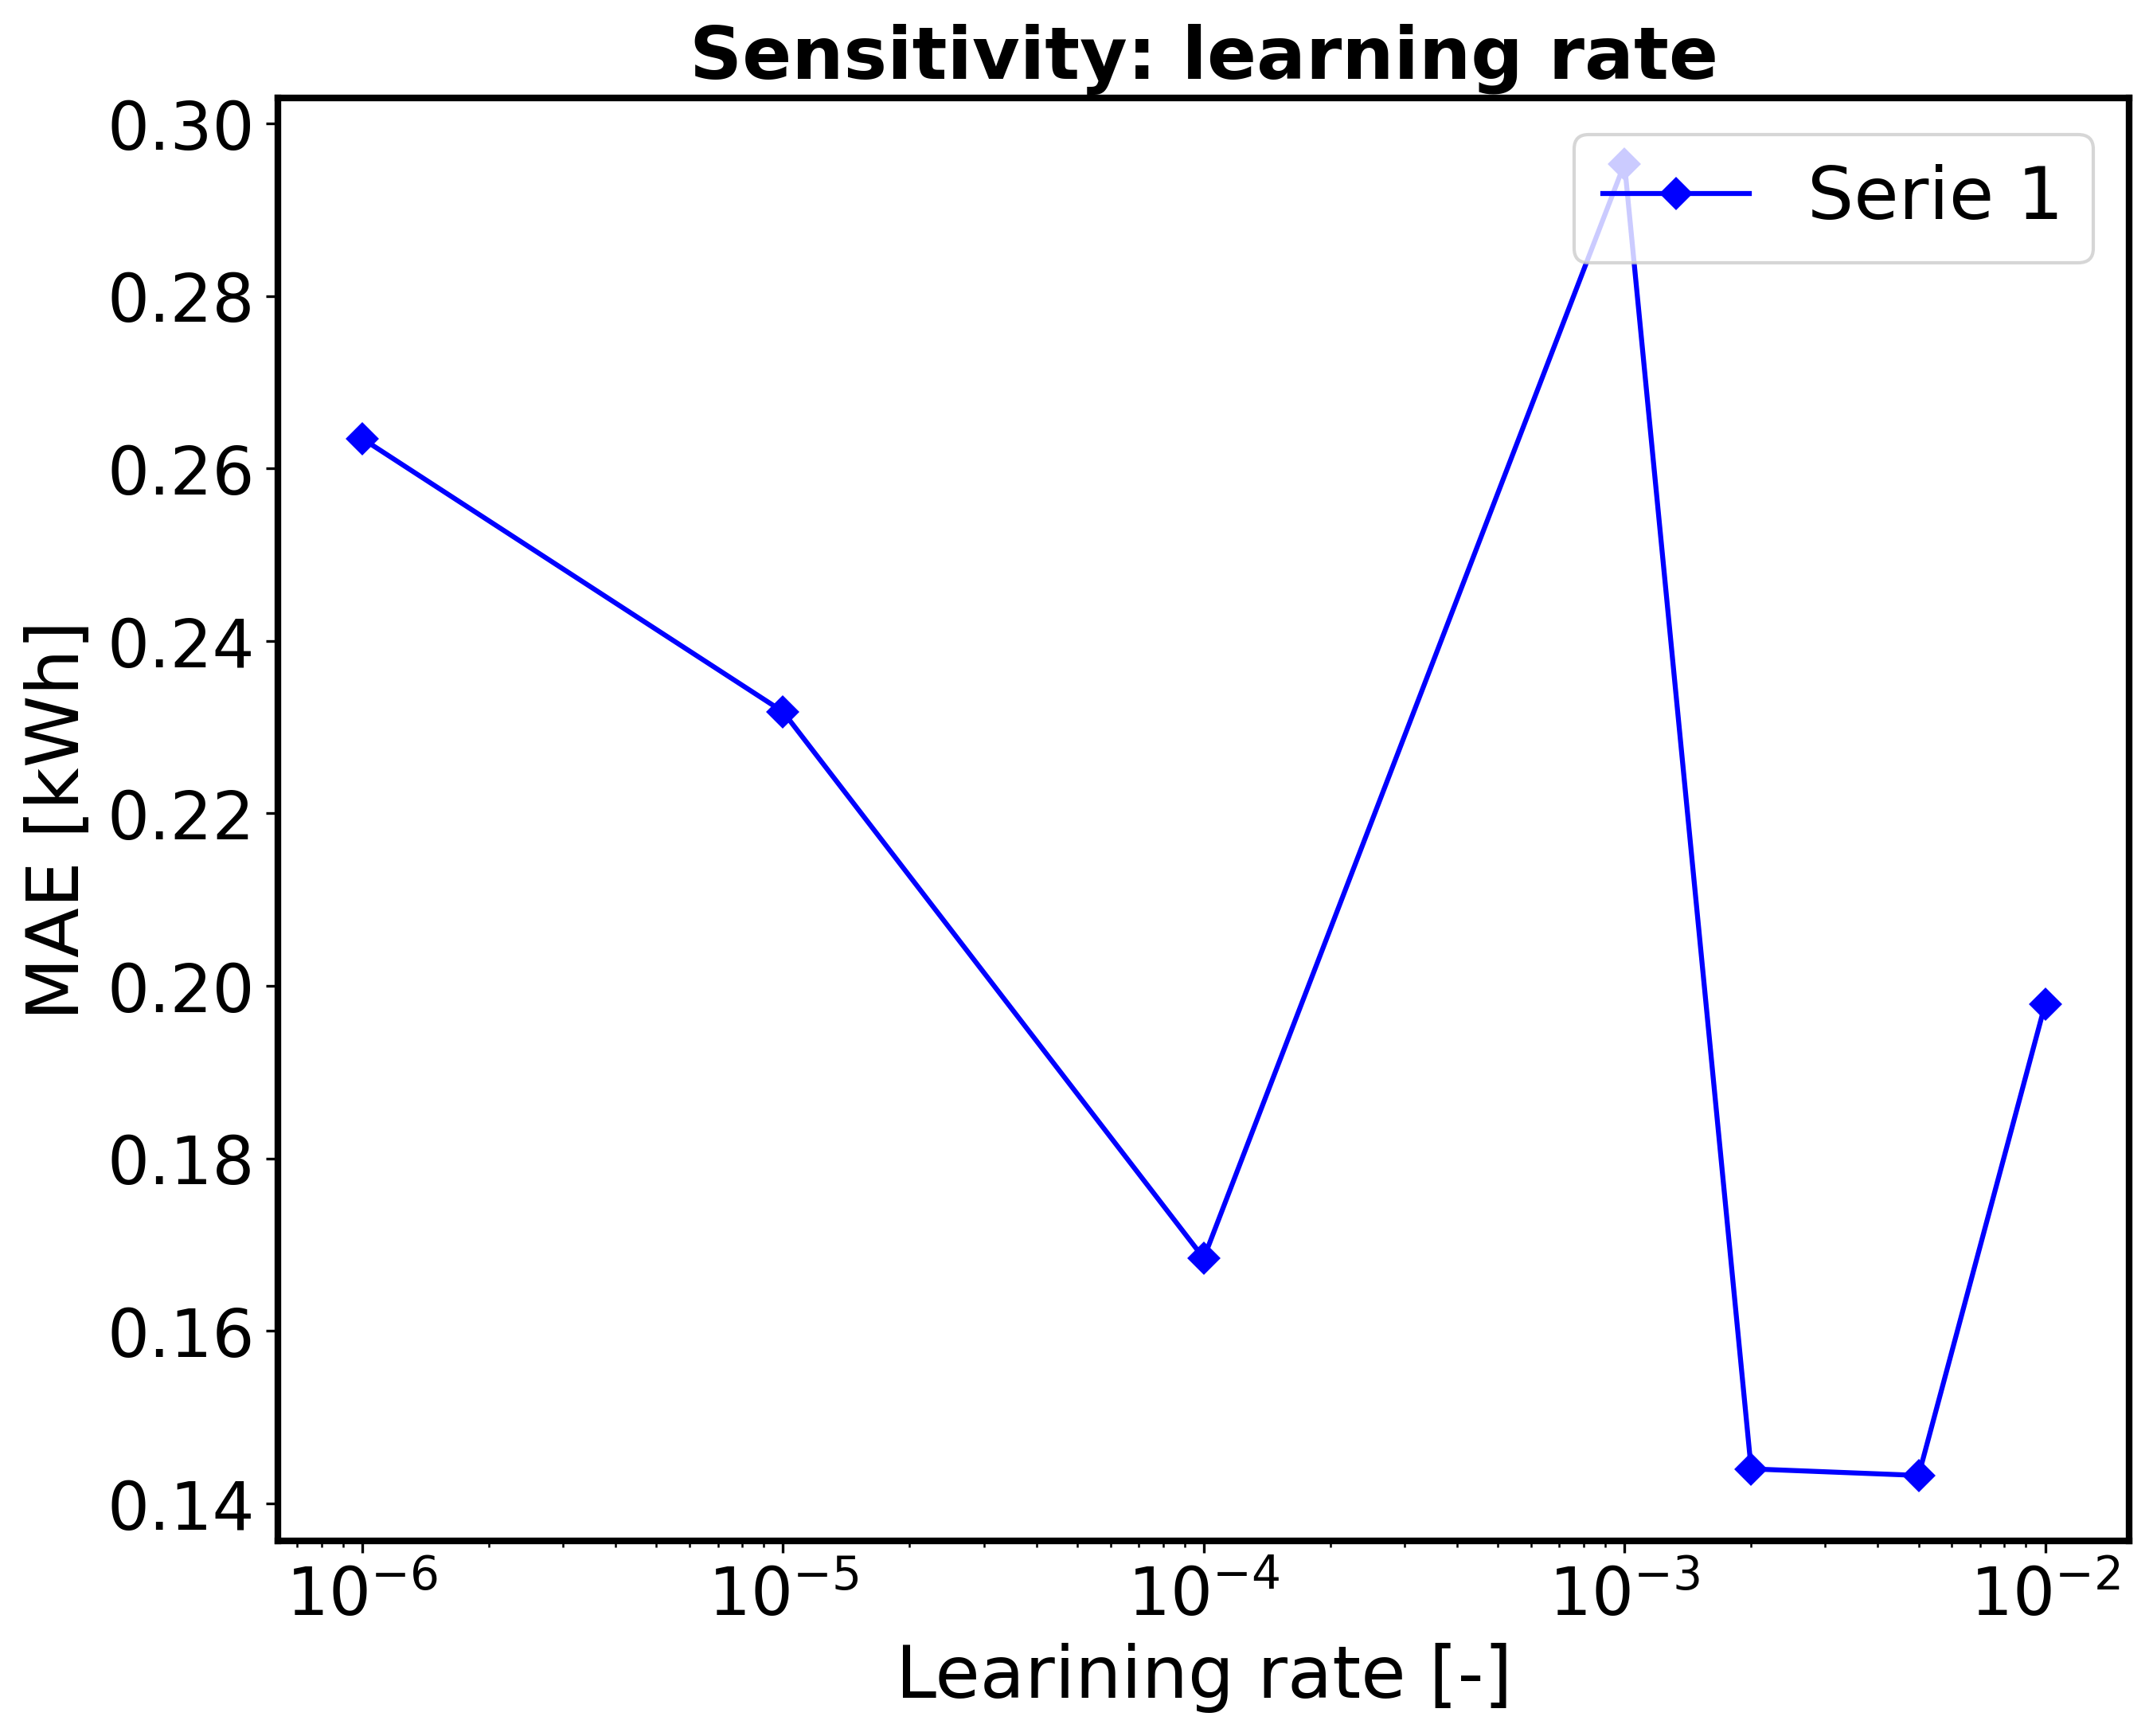
\includegraphics[width=1\linewidth]{learning_rate_serie1_model1.png}
		\caption{Model 1}
	\end{subfigure}	
	\begin{subfigure}{0.49\linewidth}
		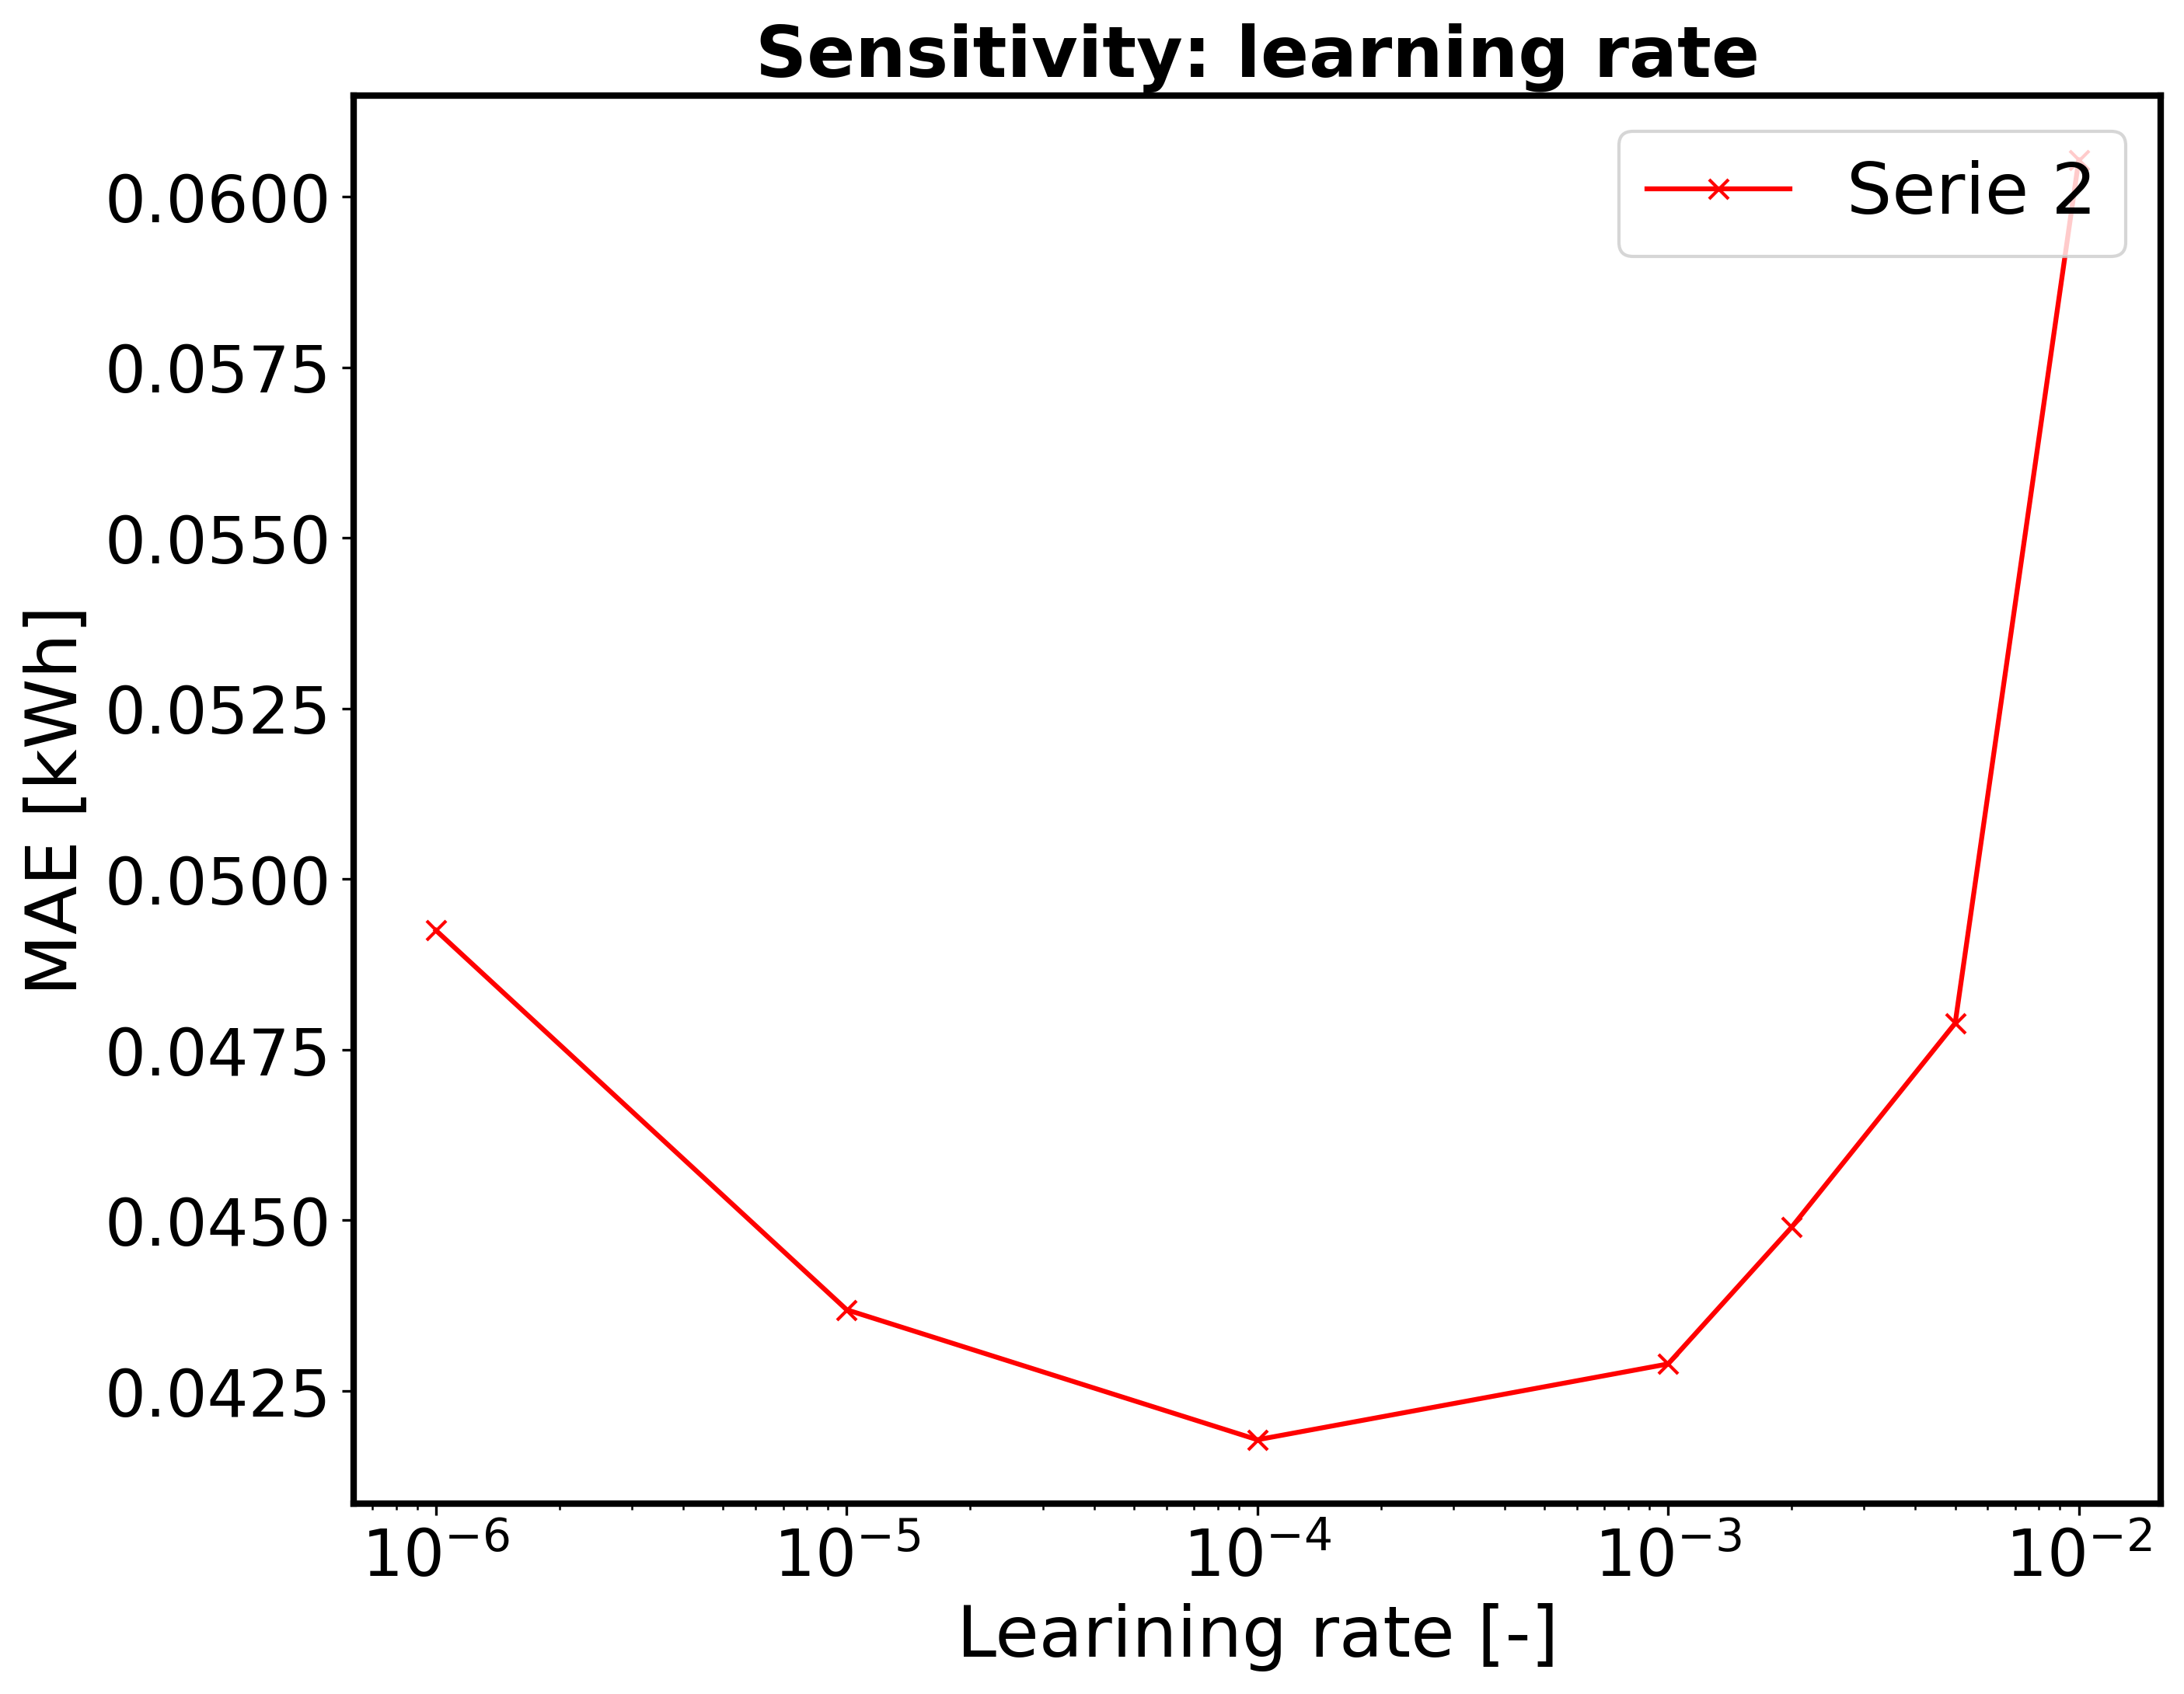
\includegraphics[width=1\linewidth]{learning_rate_serie2_model1.png}
		\caption{Model 1}
	\end{subfigure}
	\begin{subfigure}{0.5\linewidth}
		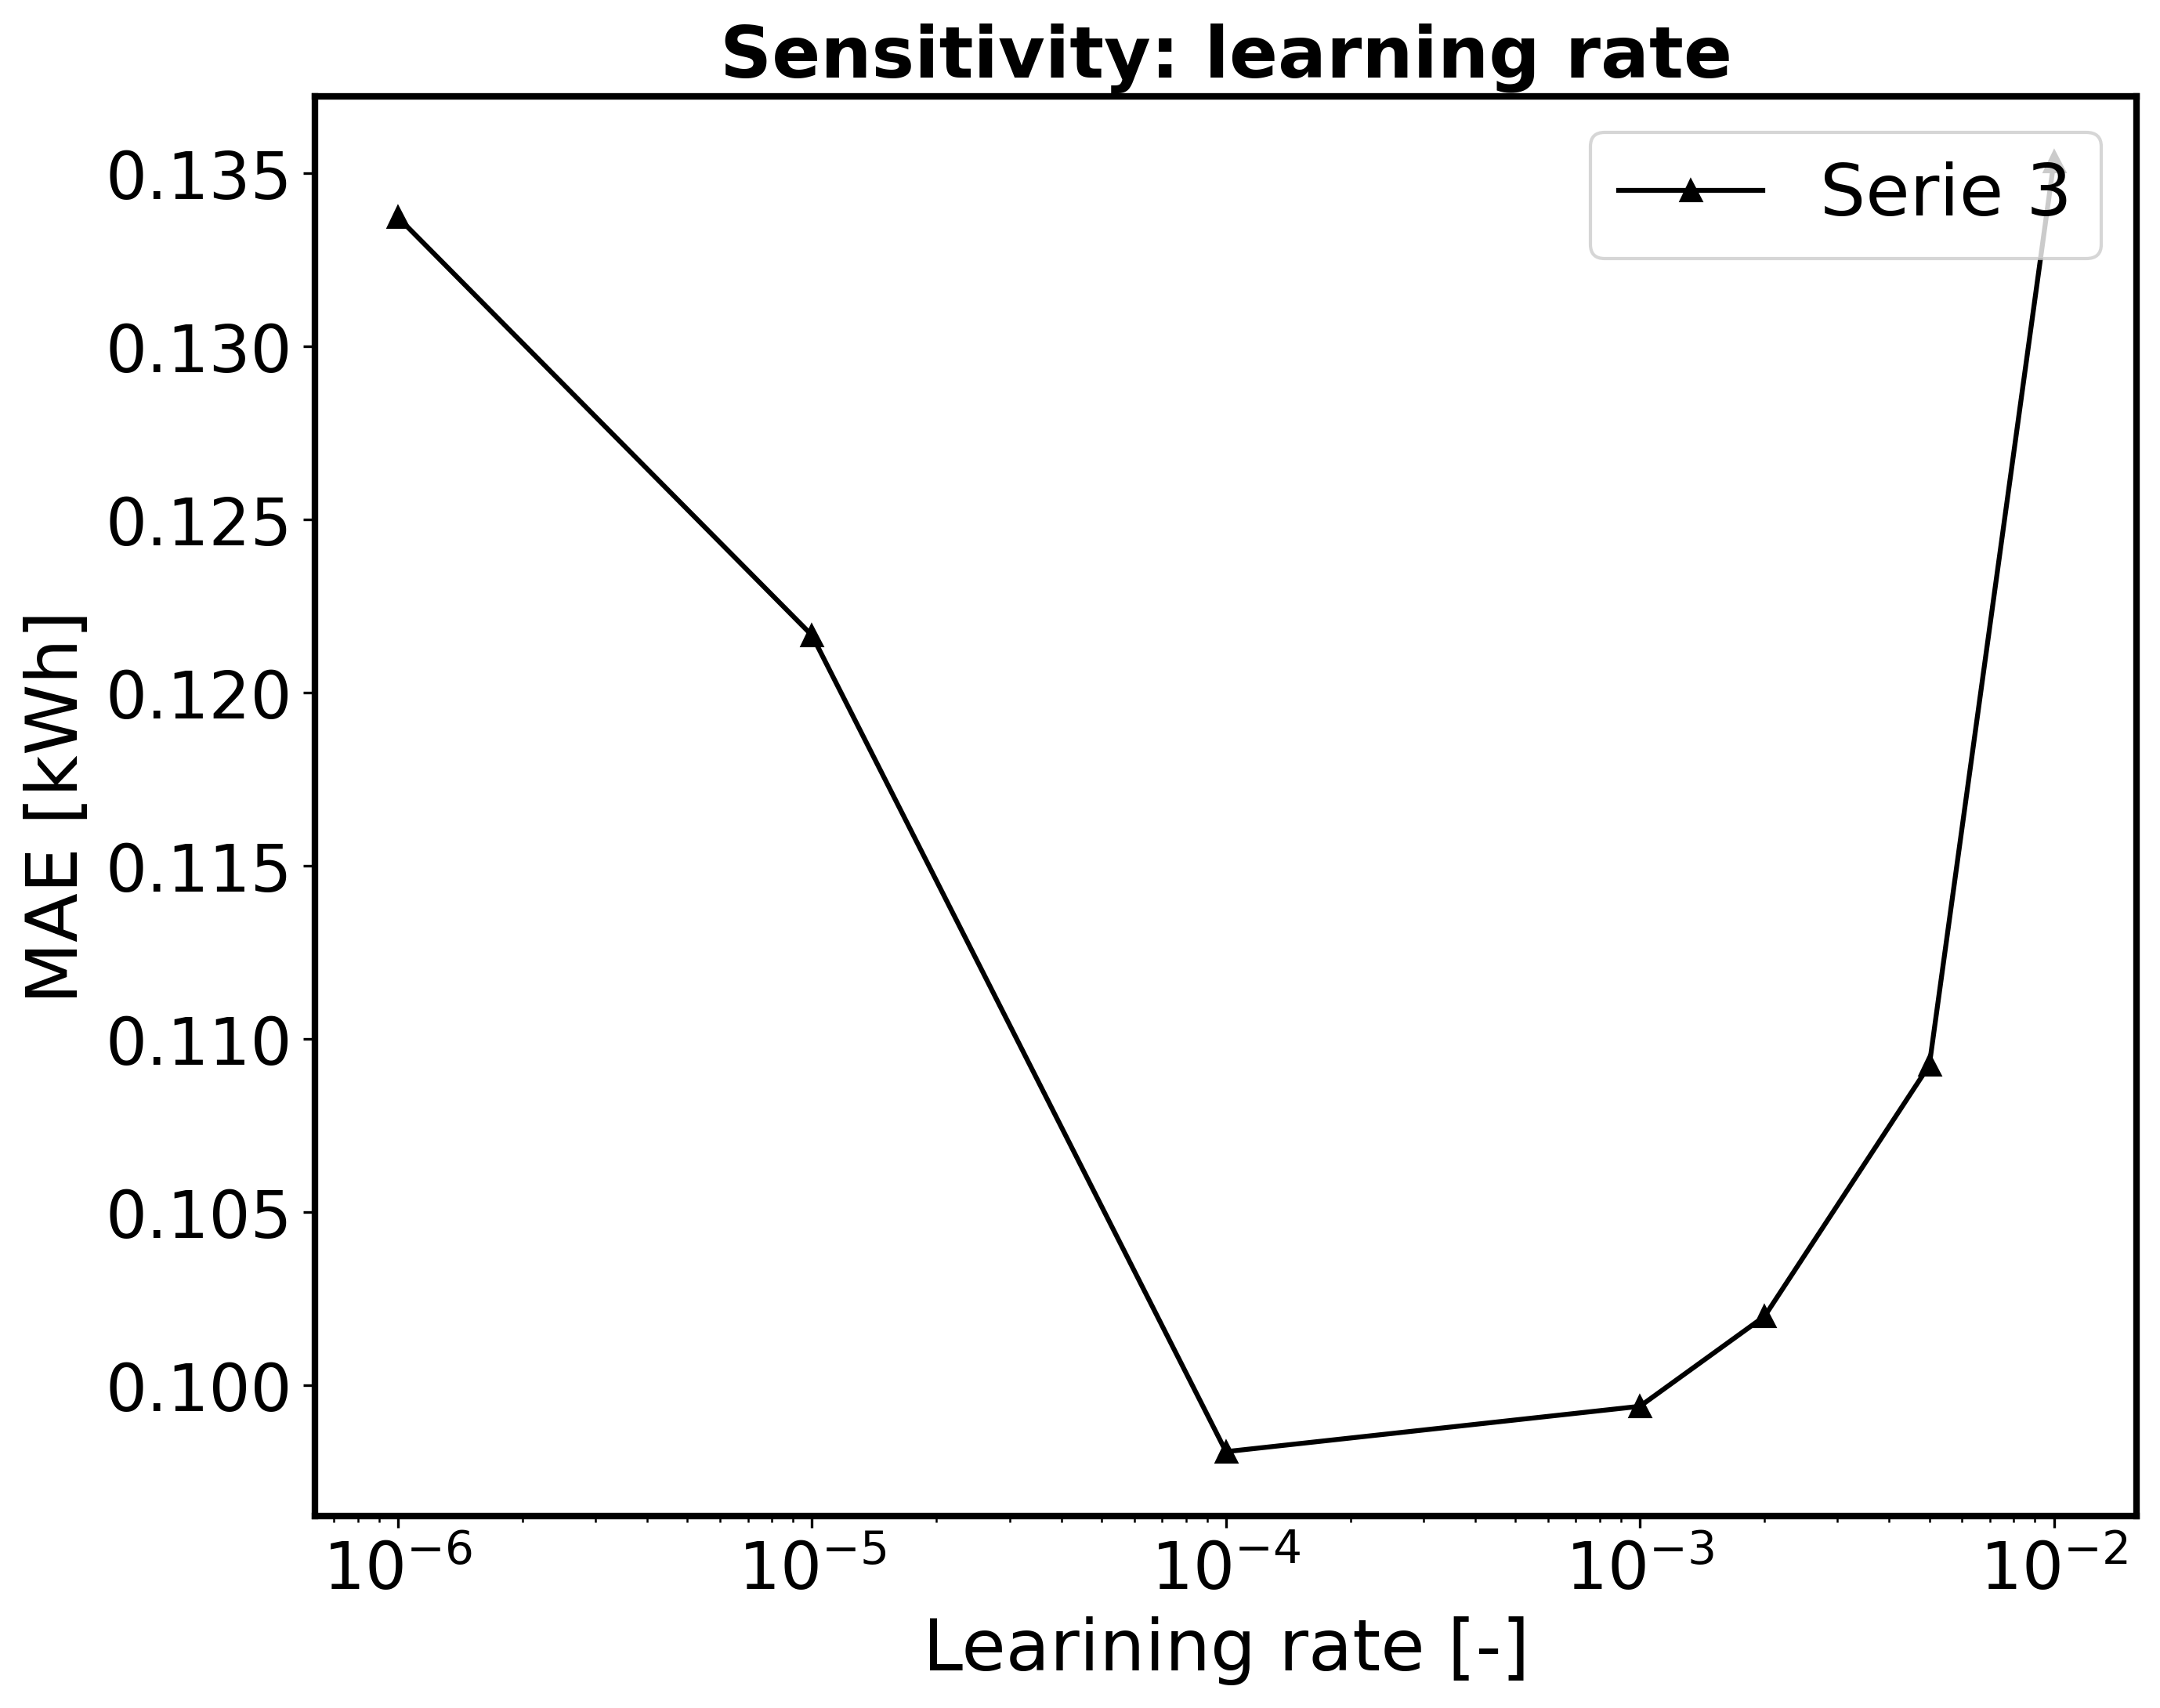
\includegraphics[width=1\linewidth]{learning_rate_serie3_model1.png}
		\caption{Model 1}
	\end{subfigure}
	\caption{The evaluation of the error on the validation set in function of the learning rate size.}
	\label{fig:learning_rate_model1}
\end{figure}


\textbf{Final model}\\
The final parameters for model one are displayed in Table \ref{tab:final_model1}.

\begin{table}[h]
	\centering
	\begin{tabular}{@{}l|ccc@{}} \toprule
		\multicolumn{4}{c}{Model 1: Stateless (no flatten layer)}\\\midrule\midrule
		\textbf{Parameters}	& \textbf{Serie $ 1 $} & \textbf{Serie $ 2 $} & \textbf{Serie $ 3 $}\\\midrule
		Units LSTM & $20 $&$ 50 $  & $50 $\\
		layers LSTM & $1 $&$ 3 $  & $3$\\
		Lag value & $96 $&$ 96$  & $48$\\
		Learning rate & $0.005 $&$ 0.0001$  & $0.0001$\\\hline
		Dropout inputs LSTM   & $ 0 $ & $ 0.2 $ & $ 0 $\\
		Dropout DENSE   & $ 0 $ & $ 0 $ & $ 0.4 $\\\bottomrule
	\end{tabular}
	\caption{Final values obtained after the parameter search for model 1.}
	\label{tab:final_model1}
\end{table}



\clearpage
\subsubsection{Model 2: Stateless with flatten layer}

\textbf{Phase 1}\\
The previous explained procedure is repeated for the other models. From Table \ref{tab:relative_performance_parameters_phase_one_model_two} it can again be seen that the choice of learning rate has the potential to give a big improvement and the use of an increased lag value of $ 96 $ didn't give a major improvement.\\ 

\textbf{Phase 2}\\
From Figure \ref{fig:sensitivity_model2} it follows that:
\begin{itemize}
	\item Serie 1: The best setting after phase one and two is when a regularization parameter on the input weigh matrices is added of $ 10^{-5} $together with $ 3 $ LSTM layers and $ 50 $ hidden states. 
	\item Serie 2: The best setting after phase one and two is when a regularization parameter on the input weigh matrices is added of $ 10^{-3} $together with $ 3 $ LSTM layers and $ 50 $ hidden states.
	\item Serie 3: The best setting after phase one and two is when a dropout rate of $ 0.4 $ is added on the dense layer together with $ 3 $ LSTM layers and $ 50 $ hidden states.
\end{itemize}

\textbf{Phase 3}\\
Figure \ref{fig:learning_rate_model2} shows the sensitivity of the size of the learning rate in function of the MAE.\\

\textbf{Final model}\\
The final parameters for model two is displayed in Table \ref{tab:final_model2}.

\begin{table}[h]
	\centering
	\begin{tabular}{@{}l|ccc@{}} \toprule
		\multicolumn{4}{c}{Model 2: Stateless (no flatten layer)}\\\midrule\midrule
		\textbf{Parameters}	& \textbf{Serie $ 1 $} & \textbf{Serie $ 2 $} & \textbf{Serie $ 3 $}\\\midrule
		Units LSTM & $50 $&$ 50 $  & $50 $\\
		layers LSTM & $3 $&$ 3 $  & $3$\\
		Lag value & $96 $&$ 48$  & $96$\\
		Learning rate & $0.002 $&$ 10^{-5}$  & $0.0001$\\\hline
		Regularization on input weigh matrices LSTM   & $ 10^{-5} $ & $ 10^{-3} $ & $ 0 $\\
		Dropout DENSE   & $ 0 $ & $ 0 $ & $ 0.4 $\\\bottomrule
	\end{tabular}
	\caption{Final values obtained after the parameter search for model 2.}
	\label{tab:final_model2}
\end{table}

\newpage
\subsubsection{Model 3: Stateful model}
The model is trained by making use of a batch size of one, which means that the weights of the LSTM block is updated by comparing each output immediately with its reference. The downside of the use of this model is that before the prediction of the consumption of a day, the model first needs to be seeded.\\

\textbf{Phase: 1}\\
During phase one the values chosen for the parameters as mentioned before, slightly different. The batch size and the lag value are both put to one. As can be seen in Figure \ref{tab:relative_performance_parameters_phase_one_model_three} the learning rate is still an important parameter to tune, but is also seen in Table \ref{tab:best_performing_para_phase1_model3} that one LSTM layer performed better than using three for the different series.\\ 

\textbf{Phase: 2}\\
From Figure \ref{fig:sensitivity_model3} it follows that:
\begin{itemize}
	\item Serie 1: The best setting during phase one as shown in Table \ref{tab:best_performing_para_phase1_model3} outperformed all settings during phase two. 
	\item Serie 2: The best setting after phase one and two is when a regularization parameter on the hidden state weigh matrices is added of $ 10^{-3} $together with $ 3 $ LSTM layers and $ 50 $ hidden states.
	\item Serie 3: The best setting during phase one as shown in Table \ref{tab:best_performing_para_phase1_model3} outperformed all settings during phase two. 
\end{itemize}

It was found that the model when the three layers are used together with $ 50 $ hidden recurrent states, often produces a very big loss during training. If this is the case, the output of the training loss becomes not a number. Only for the regularizer on the recurrent hidden states of the LSTM and the regularizer on the inputs of the LSTM the results were better. The results of the two regularizers are shown in Figure \ref{fig:sensitivity_model3}.\\

As can be seen the parameter search of phase two for serie one and two performs worse than the parameter search of phase one. It is not necessarily the case that the addition of regularizers or dropout layers is the only cause of this bad behaviour. As could be seen in Tables \ref{tab:relative_performance_parameters_phase_one_model_three} and \ref{tab:best_performing_para_phase1_model3} one layer performed often better than three layers, which could also contribute to the worst results obtained during parameter search two. Only for serie 2 the best setting of phase one is outperformed. \\

\textbf{Phase: 3}\\
Figure \ref{fig:learning_rate_model3} shows the sensitivity of the size of the learning rate in function of the MAE.\\

\textbf{Final model}\\
The final parameters for model two is displayed in Table \ref{tab:final_model3}.

\begin{table}[h]
	\centering
	\begin{tabular}{@{}l|ccc@{}} \toprule
		\multicolumn{4}{c}{Model 3: Stateful}\\\midrule\midrule
		\textbf{Parameters}	& \textbf{Serie $ 1 $} & \textbf{Serie $ 2 $} & \textbf{Serie $ 3 $}\\\midrule
		Units LSTM & $50 $&$ 50 $  & $20 $\\
		layers LSTM & $1 $&$ 3 $  & $1$\\
		Lag value & $1 $&$ 1$  & $1$\\
		Learning rate & $10^{-4} $&$10^{-6} $  & $10^{-4} $\\\hline
		Regularization on hidden states weigh matrices LSTM  & $ 0 $ & $ 10^{-3} $ & $ 0 $\\\bottomrule
	\end{tabular}
	\caption{Final values obtained after the parameter search for model 2.}
	\label{tab:final_model3}
\end{table}




\section{Conclusion}
This chapter discussed the data to perform the daily electricity consumption forecast on and which models are used. First, the baseline models were discussed. It was found that the mean forecast performed best for the error metrics: MAE, MSE, NRMSE and RMSE. ``MAPE forecast'' performed best when the MAPE error metric was considered. Both models predict the trend line and don't predict peaks in contrary to the closest day, 1 day and 7 days models. Next, the LSTM models that were developed were discussed. This included the practical considerations of the implementation of the models in Keras and a parameter search. The parameter search was done in three phases in order to reduce calculation load. It was found that the learning rate was the parameter that contributed the most to model performance.


%%% Local Variables: 
%%% mode: latex
%%% TeX-master: "thesis"
%%% End: 
